\documentclass{assignment}

\usepackage{float}
\usepackage{tikz}
\usepackage{adjustbox}
\usepackage{titlesec}
\usepackage{soul}
\usepackage{csvsimple}

\usepackage{graphicx}
\usepackage{subcaption}
\usetikzlibrary{shapes, arrows}

\usetikzlibrary{calc,patterns,angles,quotes}
\setlength{\parindent}{0pt}

\hypersetup{
pdftitle={Advanced Dynamics of Mechanical Systems},
pdfsubject={Report for assignment 2},
pdfauthor={Tommaso Bocchietti}
}

\makeglossaries

% \newacronym{cfd}{CFD}{Computational Fluid Dynamics}

\begin{document}

\title{Advanced Dynamics of Mechanical Systems \\ Assignment 2}
\author{Tommaso Bocchietti 10740309 \\ Nome Cognome Codice Persona \\ Nome Cognome Codice Persona}
\date{A.Y. 2023/24}

\maketitle

\begin{figure}[H]
    \centering
    
\includegraphics[width=0.7\textwidth]{./pdf/Polimi_logo_coverpage.pdf}
    \label{fig:Polimi_logo}
\end{figure}

\clearpage
\tableofcontents
\listoffigures
\listoftables
% \lstlistoflistings
% \printglossary[type=\acronymtype]

\clearpage
\section{Requests}
\label{sec:requests}

A system of two aluminum bars of the same material is shown in the following figure.
The system is subjected to two external loads, $P_x$ and $P_y$, at joint B.
A and C are connected to pinned supports.

\begin{figure}[h]
    \centering
    \begin{tikzpicture}[scale=3]

        \coordinate (A) at (0,0.5);
        \coordinate (B) at (3,0.5);
        \coordinate (Bf) at (3.7,1);
        \coordinate (C) at (3,0);

        % Joint names
        \node at (A) [above, left] {A};
        \node at (B) [below, above] {B};
        \node at (C) [below, left] {C};

        % Initial position
        \draw (A) -- (B) node[midway, below] {$L_1$};
        \draw (C) -- (B) node[midway, left] {$L_2$};

        % Deformed position
        \draw[dashed] (A) -- (Bf)node[midway, above] {$l_1$};
        \draw[dashed] (C) -- (Bf)node[midway, right] {$l_2$};

        % Labels
        \pic [draw, ->, "$\alpha$", angle radius=2cm] {angle = B--A--Bf};
        \pic [draw, <-, "$\beta$", angle radius=0.7cm] {angle = Bf--C--B};

        % Support at the end of Beam 1
        \draw[fill] (0,0.5) circle (0.03);

        % Support at the end of Beam 2
        \draw[fill] (3,0) circle (0.03);

        % Arrows at coordinate Bf
        \draw[->] (Bf) -- ++(0.3, 0) node[right] {$\vec{P_x}$};
        \draw[->] (Bf) -- ++(0, 0.3) node[above] {$\vec{P_y}$};
        \draw[->] (B) -- (Bf) node[midway, above] {$\vec{u}$};
        % \draw[->, shorten >=150pt] (Bf) -- (A) node[above, above] {$\vec{F_1}$};
        % \draw[->, shorten >=50pt] (Bf) -- (C) node[above, right] {$\vec{F_2}$};

    \end{tikzpicture}
    \caption{Problem representation}
    \label{fig:problem_representation}
\end{figure}

The problem asks to:

\begin{itemize}
    \item Obtain the external loads $P_x$ and $P_y$ as a function of horizontal and vertical displacements at point B (namely $u$ and $v$).
    \item Determine the displacements in both $x$ and $y$ directions for $1000$ load increments of $+5\text{N}$ for both $P_x$ and $P_y$ (from zero).
    \item Find the displacement of point B after the final increment.
\end{itemize}

Write a \texttt{MATLAB} code with a convergence error of $10^-5$ to numerically solve the problem.
Use a combination of (a) Euler and N-R, and (b) Euler and modified N-R.
Also plot the resultant force versus the resultant displacement.

Use the Green strain measure:

\begin{equation}
    E_i = \frac{l_i^2 - L^2}{2L^2}
    \label{eq:green_strain_measure_formula}
\end{equation}

From now on, we will refer to the Green strain measure as $\epsilon_{1,2}$ to differentiate it from the Young's modulus $E_{1,2}$.

\begin{table}[H]
    \centering
    \begin{tabular}{|c|c|c|}
        \hline
        \textbf{Parameter} & \textbf{Value} & \textbf{Unit} \\ \hline
        $E_1 = E_2 = E$    & $70$           & $\text{GPa}$  \\ \hline
        $L_1$              & $3$            & $\text{m}$    \\ \hline
        $L_2$              & $0.5$          & $\text{m}$    \\ \hline
        $A_1 = A_2 = A$    & $0.0001$       & $\text{m}^2$  \\ \hline
    \end{tabular}
    \caption{Parameters of the system}
    \label{tab:parameters_of_the_system}
\end{table}

\section{FE model}
\label{sec:FE_model}

In the following subsections, we will describe the Finite Element Model (FEM) of the harbour crane and discuss some key aspects of the model, such as the geometry and material properties and the assembly of the mass and stiffness matrices.
We will also discuss the results obtained from the modal analysis of the system.

\subsection{Geometry and material properties}
\label{sub:geometry_and_material_properties}

At first the FEM model was created considering a safety factor of $2$ and a maximum operating frequency range of $0-8 [Hz]$.

From theory, we know that in a FEM model the geometry and in particular the length of the elements is determinant when it comes to the accuracy of the results, given that a too coarse mesh can lead to inaccurate results, while a too fine mesh can lead to a high computational cost.
Because of this, the maximum length of the single elements was determined as:

\begin{equation}
    L_{\text{max}} = \sqrt{\frac{\pi^2}{\eta \Omega_{max}} \sqrt{\left(\frac{EJ}{m}\right)_{min}}} \approx 12 \quad [m]
\end{equation}

Once the model has been discretized and the geometrical and material properties have been assigned to each element based on the suggested values reported in Table \ref{tab:parameters}, the model was imported in adequate \texttt{MATLAB} data structures.

The output of this first step is a schematized version of the harbour crane, as shown in Figure \ref{fig:harbour-crane-scheme}.

\begin{figure}[H]
    \centering
    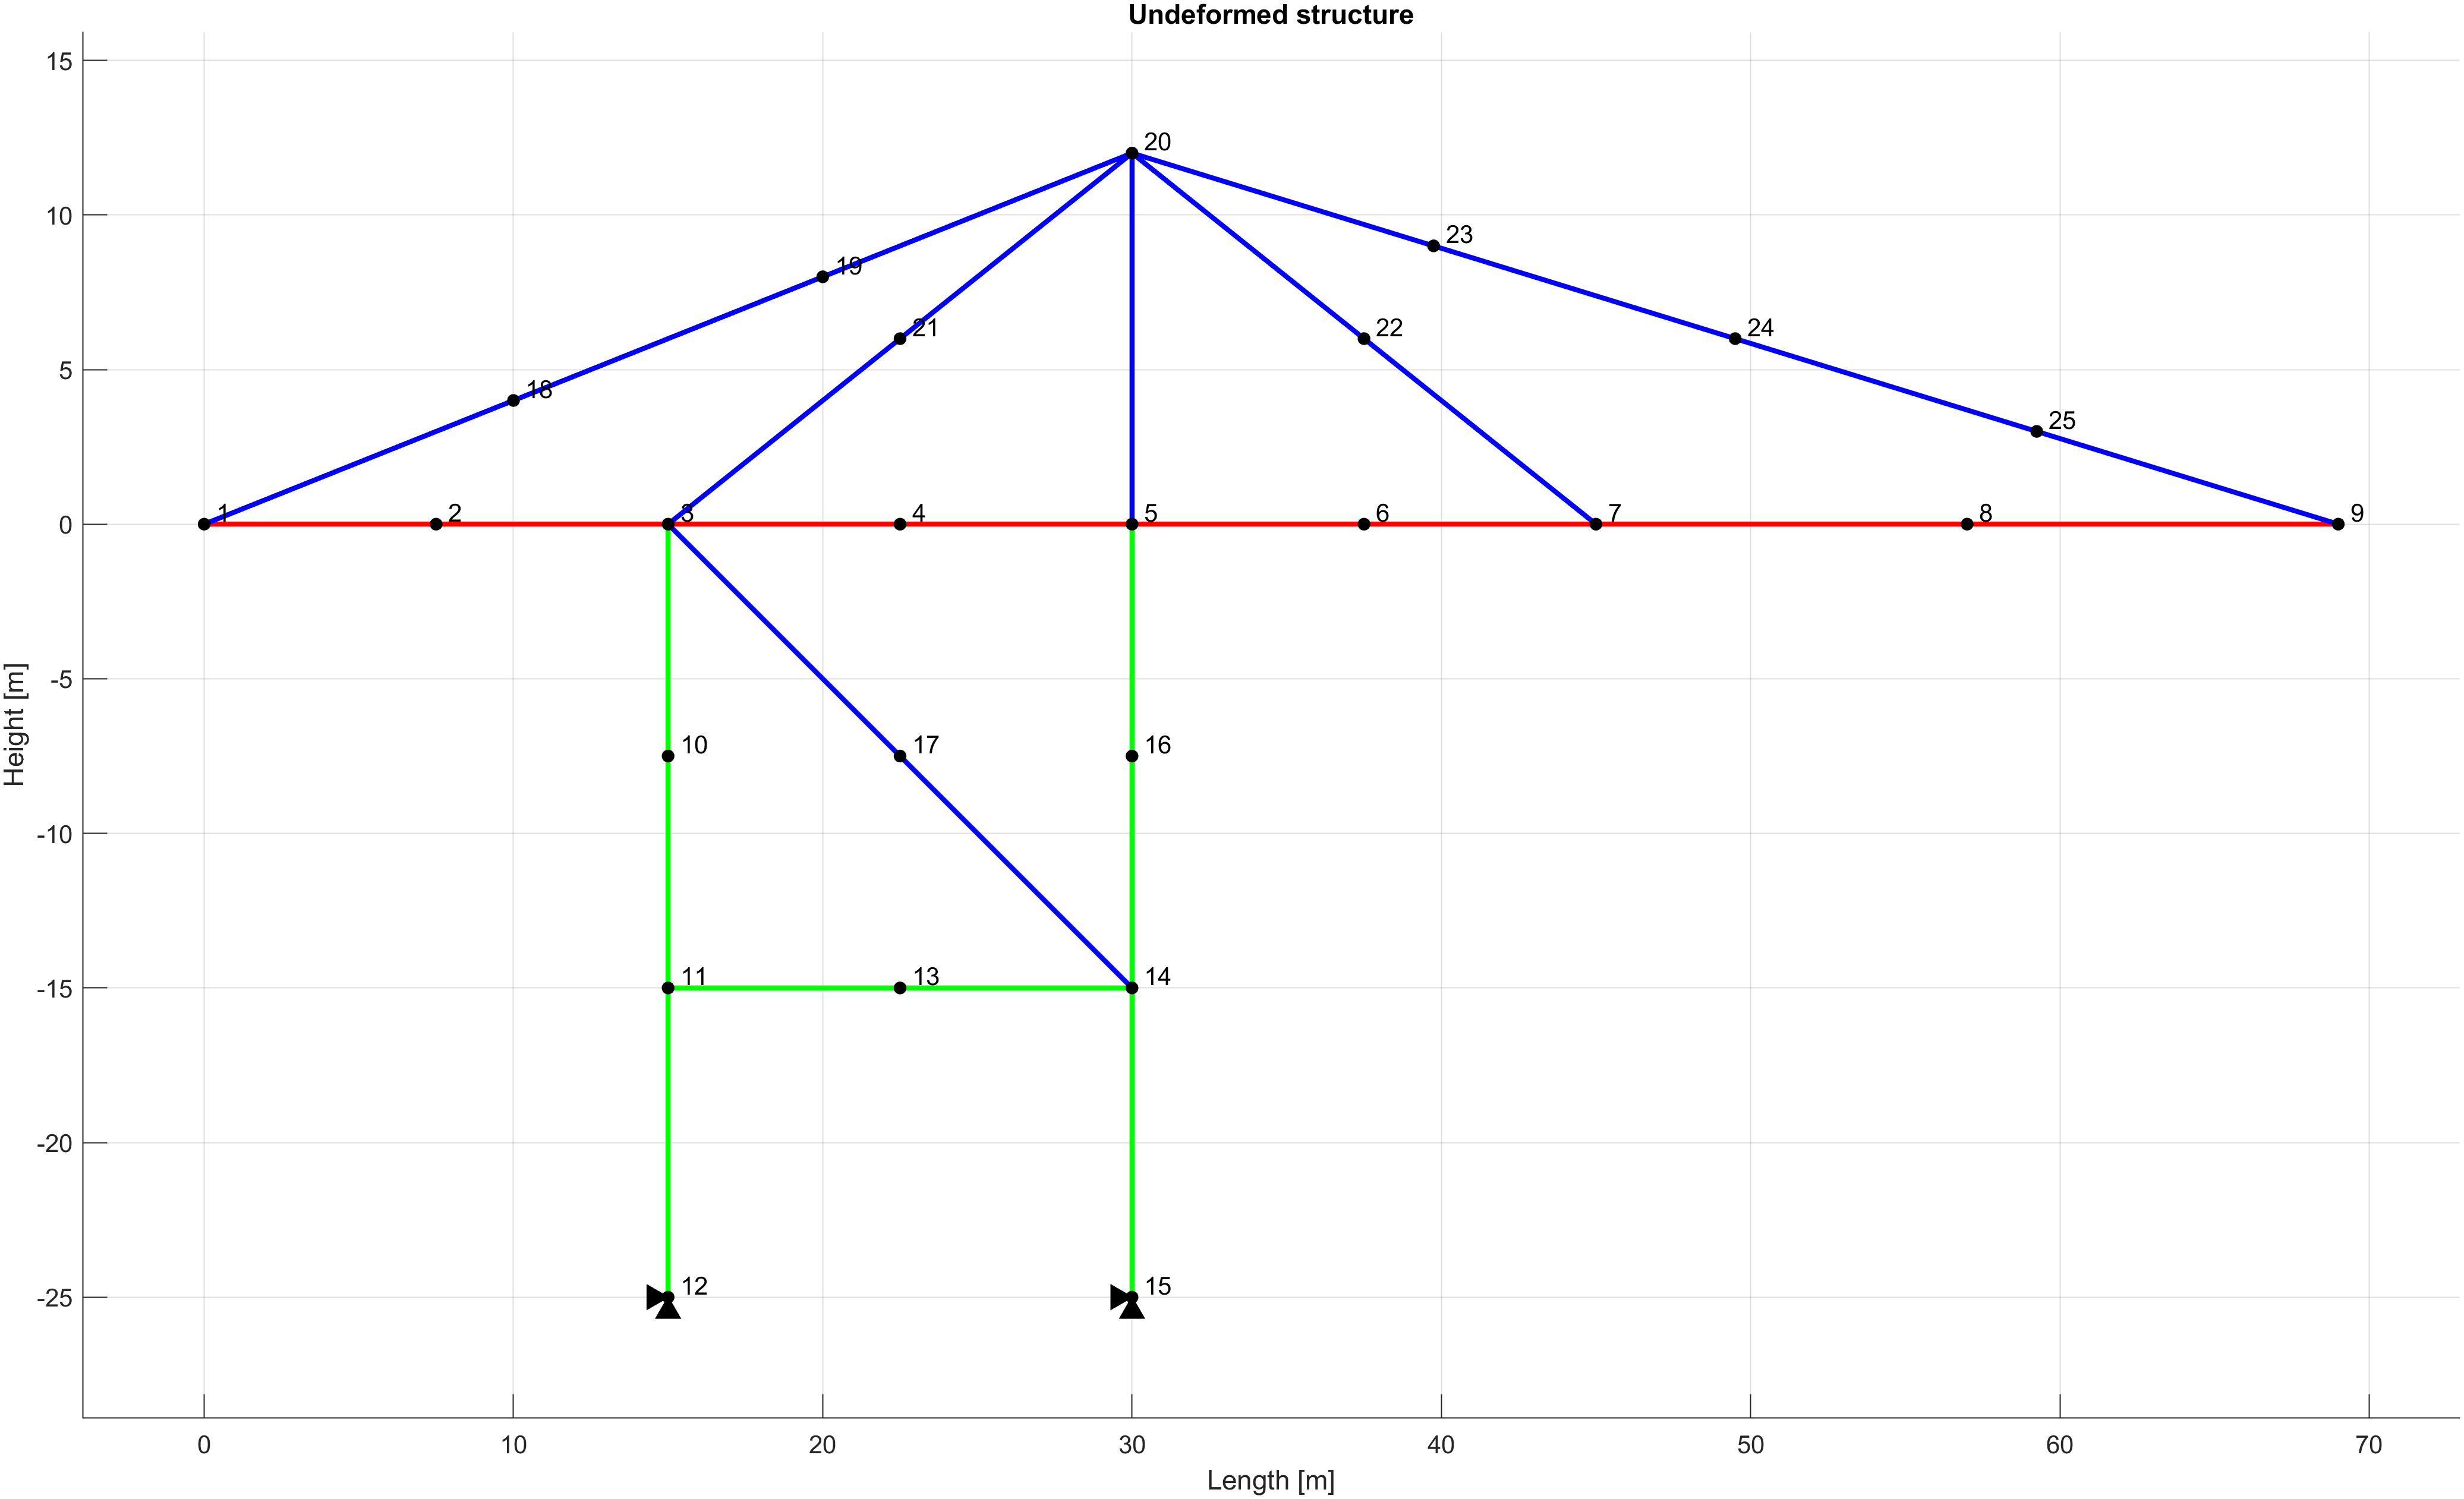
\includegraphics[width=0.7\textwidth]{img/MATLAB/undeformed-structure.png}
    \caption{Harbour crane scheme. Node naming: [\textbf{A}, \textbf{B}, \textbf{C}, \textbf{D}, \textbf{O2}] = [\textbf{\#9}, \textbf{\#14}, \textbf{\#1}, \textbf{\#7}, \textbf{\#15}]}
    \label{fig:harbour-crane-scheme}
\end{figure}

As suggested/requested by the assignment, the harbour crane was modelled as a 2D frame structure composed of beam elements.
As an assumption, the joints \textbf{A} and \textbf{C} were assumed to be rigid connections, even if in reality those elements are usually not capable of transmit bending moments, but only axial forces (hinge connections type).
This assumption was made to simplify the model and the analysis.
However, the model could be easily modified to include the possibility of free relative rotations in those joints by adding another degree of freedom to the system.

With respect to the schematic representation of the crane of Figure \ref{fig:harbour-crane-scheme}, the parameters of the structure are provided in Table \ref{tab:parameters}.

\begin{table}[H]
    \centering
    \begin{tabular}{|r|c|c|c|}
        \hline
        ~           & \textbf{m [kg/m]} & \textbf{EA [N]} & \textbf{EJ [Nm$^2$]} \\
        \hline
        Red beams   & $312$             & $8.2E9$         & $1.4E9$              \\
        Green beams & $200$             & $5.4E9$         & $4.5E8$              \\
        Blue beams  & $90$              & $2.4E9$         & $2.0E8$              \\
        \hline
    \end{tabular}
    \caption{Parameters of the structure}
    \label{tab:parameters}
\end{table}

For the rest of the analysis, we will assume a proportional damping matrix $[C] = \alpha [M] + \beta [K]$ with $\alpha = 0.01 [\frac{1}{s}]$ and $\beta = 2E-4 [s]$
\subsection{Matrices assembly}
\label{sub:matrices_assembly}

Once the geometrical and material properties of the structure are known, it is possible to assemble the mass and stiffness matrices of the system, and empirically also the damping matrix.

A common approach to assemble the mass and stiffness matrices is to loop over all the elements of the structure and to add the contribution of each element to the global matrices.
To do so, it is necessary to calculate the element matrices, which are the mass and stiffness matrices of each element in the local reference frame.
Then, the element matrices are transformed into the global reference frame and added to the global matrices.

The mass matrix of an element is calculated as:

\begin{equation}
    [M_{el}] = \int_{0}^{L} \rho A N^T N dx
\end{equation}

Where $\rho$ is the mass density of the material, $A$ is the cross-sectional area of the element, $N$ is the shape function matrix, and $L$ is the length of the element.

The stiffness matrix of an element is calculated as:

\begin{equation}
    [K_{el}] = \int_{0}^{L} [E] B^T B dx
\end{equation}

Where $[E]$ is the elasticity matrix of the material, $B$ is the strain-displacement matrix, and $L$ is the length of the element.

Once the element matrices are calculated, they are transformed into the global reference frame using the transformation matrix $[Q]$:

\begin{align}
    [M_{el}] & = [Q]^T [M_{el}] [Q] \\
    [K_{el}] & = [Q]^T [K_{el}] [Q]
\end{align}

Where $[Q]$ is the transformation matrix of the element, which is calculated as:

\begin{equation}
    [Q] = \begin{bmatrix}
        \cos(\theta)  & \sin(\theta) & 0 & 0             & 0            & 0 \\
        -\sin(\theta) & \cos(\theta) & 0 & 0             & 0            & 0 \\
        0             & 0            & 1 & 0             & 0            & 0 \\
        0             & 0            & 0 & \cos(\theta)  & \sin(\theta) & 0 \\
        0             & 0            & 0 & -\sin(\theta) & \cos(\theta) & 0 \\
        0             & 0            & 0 & 0             & 0            & 1 \\
    \end{bmatrix}
\end{equation}

Where $\theta$ is the angle between the local and global reference frames.

Finally, the element matrices are added to the global matrices considering the contribution of each element to the corresponding global degrees of freedom of the system:

\begin{align}
    [M] & = [M] + [Q]^T [M_{el}] [Q] \\
    [K] & = [K] + [Q]^T [K_{el}] [Q]
\end{align}

The damping matrix can be calculated similarly, using the proportional damping matrix $[C] = \alpha [M] + \beta [K]$.

\paragraph{Matrices partitioning}

As a preference choice (even if not strictly necessary), the structure geometry definition, and in particular the node and degree of freedom numbering were performed in order to have the following partitioning of the matrices:

\begin{equation}
    [M] = \begin{bmatrix}
        [M_{FF}] & [M_{FC}] \\
        [M_{CF}] & [M_{CC}] \\
    \end{bmatrix}
    \quad
    [K] = \begin{bmatrix}
        [K_{FF}] & [K_{FC}] \\
        [K_{CF}] & [K_{CC}] \\
    \end{bmatrix}
    \quad
    [C] = \begin{bmatrix}
        [C_{FF}] & [C_{FC}] \\
        [C_{CF}] & [C_{CC}] \\
    \end{bmatrix}
\end{equation}

Where the subscripts $F$ and $C$ refer to the free and constrained degrees of freedom, respectively.

\subsection{Modal analysis}
\label{sub:modal_analysis}

To understand how the structure behaves when excited by a force, it is necessary to calculate the natural frequencies and the mode shapes of the system.

As usual, the natural frequencies are the eigenvalues of the system, while the mode shapes are the eigenvectors.
Since we are dealing with a discretized system, we can expect as many natural frequencies as the number of degrees of freedom of the system.

In this phase, we can ignore the damping matrix, since its contribution is negligible in the calculation of the natural frequencies and mode shapes, so that the eigenvalues problem to be solved became:

\begin{equation}
    [M] \ddot{X} + [0] \dot{X} + [K] X = 0
\end{equation}

Which indeed brings to the standard eigenvalues problem:

\begin{equation}
    (\omega^2 [I] - [M_{FF}]^{-1} [K_{FF}]) X = 0
\end{equation}

Solvable in \texttt{MATLAB} with the following code:

\begin{lstlisting}[language=Matlab]

    [M, K] = assembly(incid, l, m, EA, EJ, gamma, idb);
    C = 1e-1 * M + 2.0e-4 * K;

    M_FF = M(1:ndof, 1:ndof);
    C_FF = C(1:ndof, 1:ndof);
    K_FF = K(1:ndof, 1:ndof);

    [mode_shapes, omega_square] = eig(M_FF\K_FF);
    omega_nat = sqrt(diag(omega_square));

\end{lstlisting}

As we have said before, from the code above we expect to have as many natural frequencies as the number of degrees of freedom of the system.
However, we always have to keep in mind the real physical representation of the problem.
In this case, the model represents a crane, which is a machine that typically works or is subjected to forces having a low frequency range.
As suggested by the assignment, our interest is in the $0-8 [Hz]$ frequency range.

Therefore, it's reasonable to expect that just the firsts few natural frequencies are significant, while for the others (even if present also in the real structure) is difficult that they will be excited by the forces acting on the crane and so we can consider them as negligible.

In the following, we will show the first four mode shapes of the system and the corresponding natural frequencies.

\begin{figure}[H]
    \begin{minipage}[b]{0.45\textwidth}
        \centering
        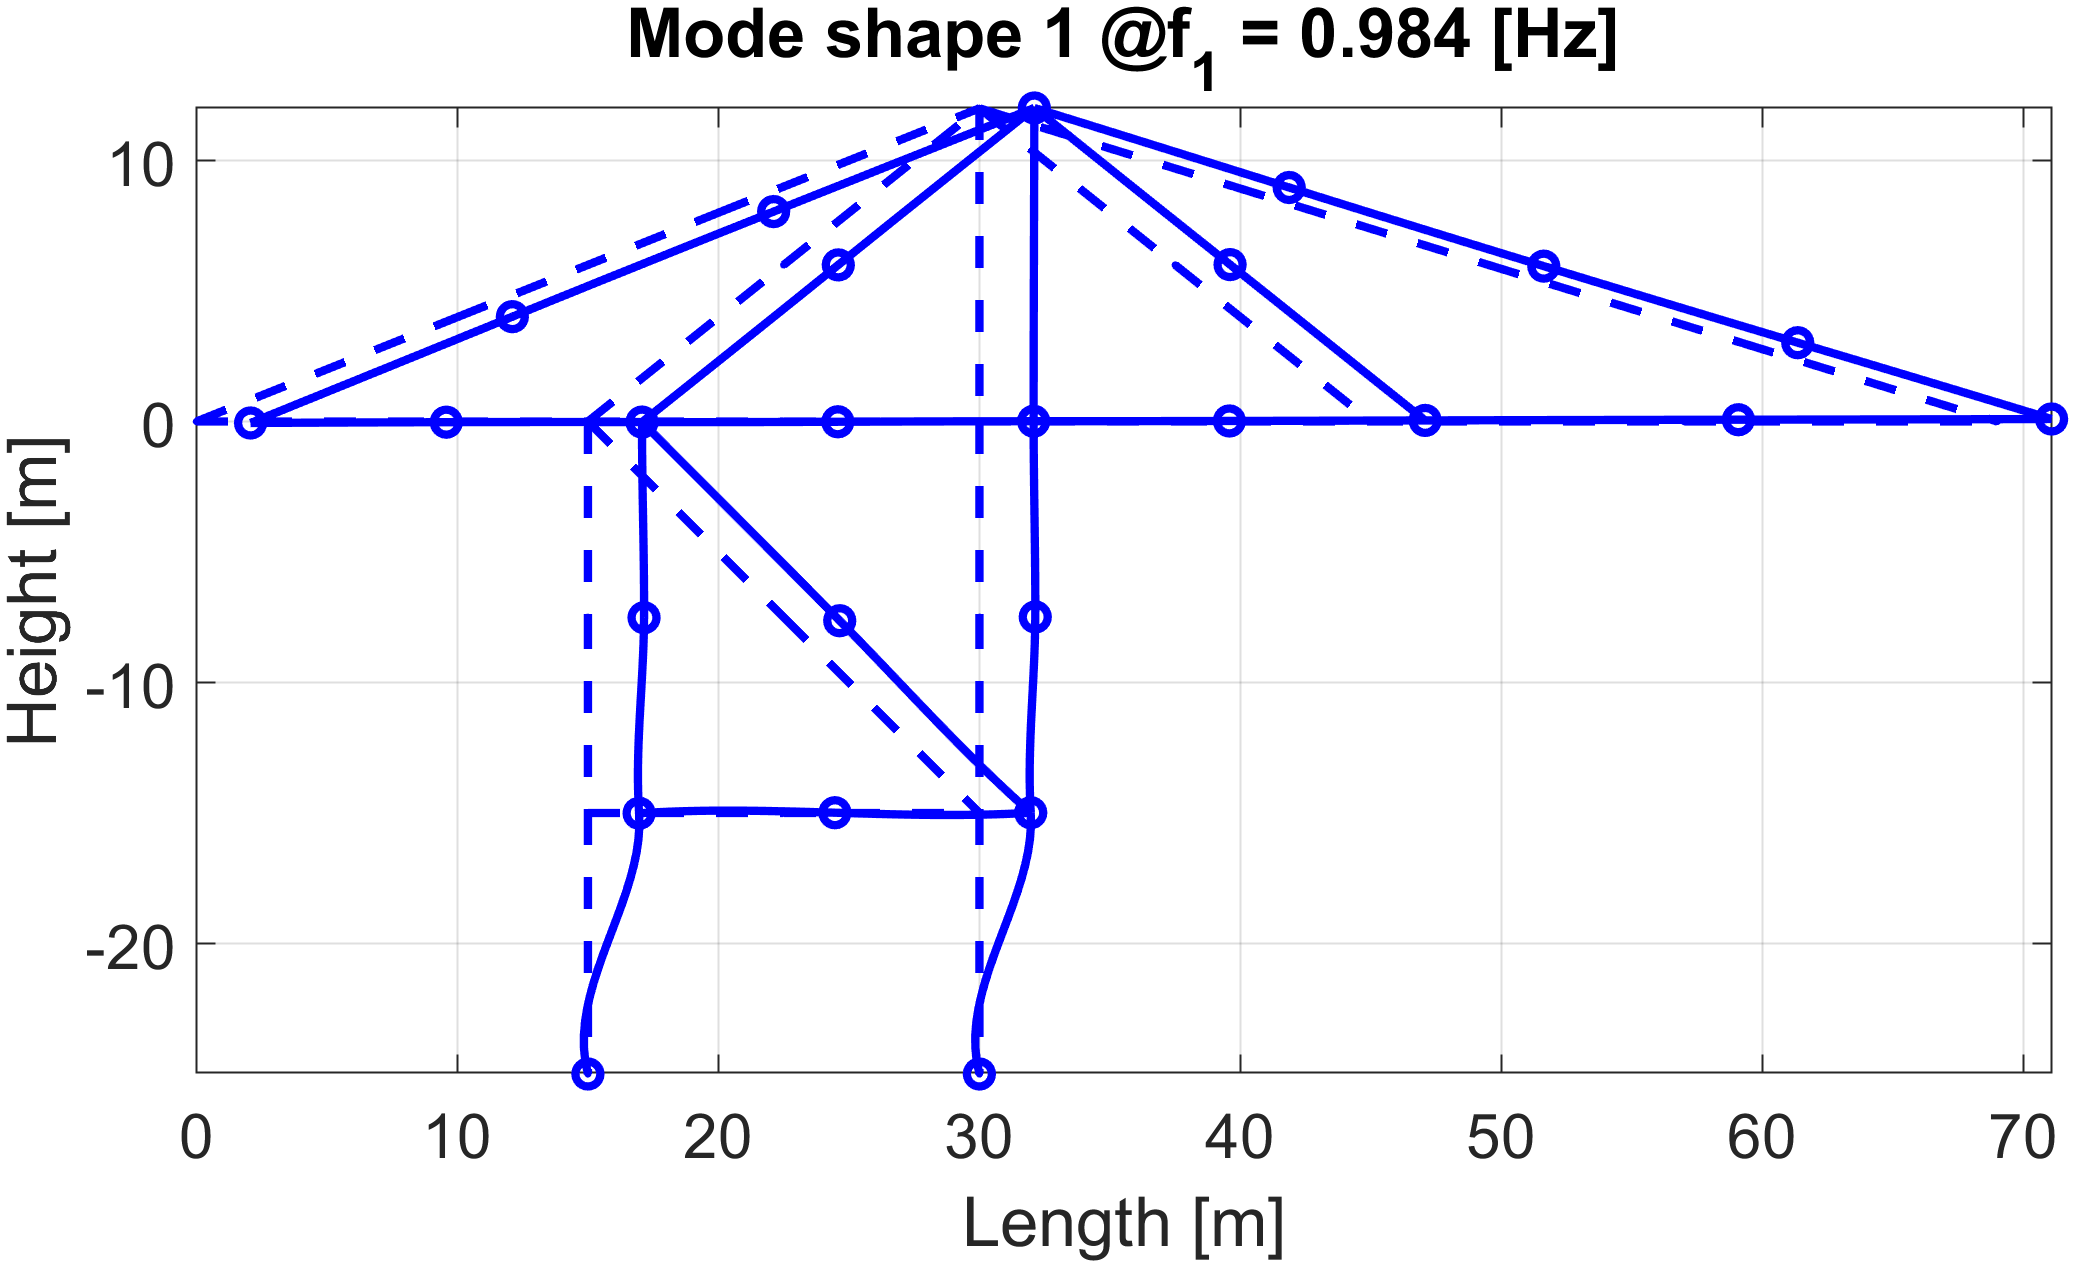
\includegraphics[width=\textwidth]{img/MATLAB/ModeShapes/Mode_01.png}
    \end{minipage}
    \hfill
    \begin{minipage}[b]{0.45\textwidth}
        \centering
        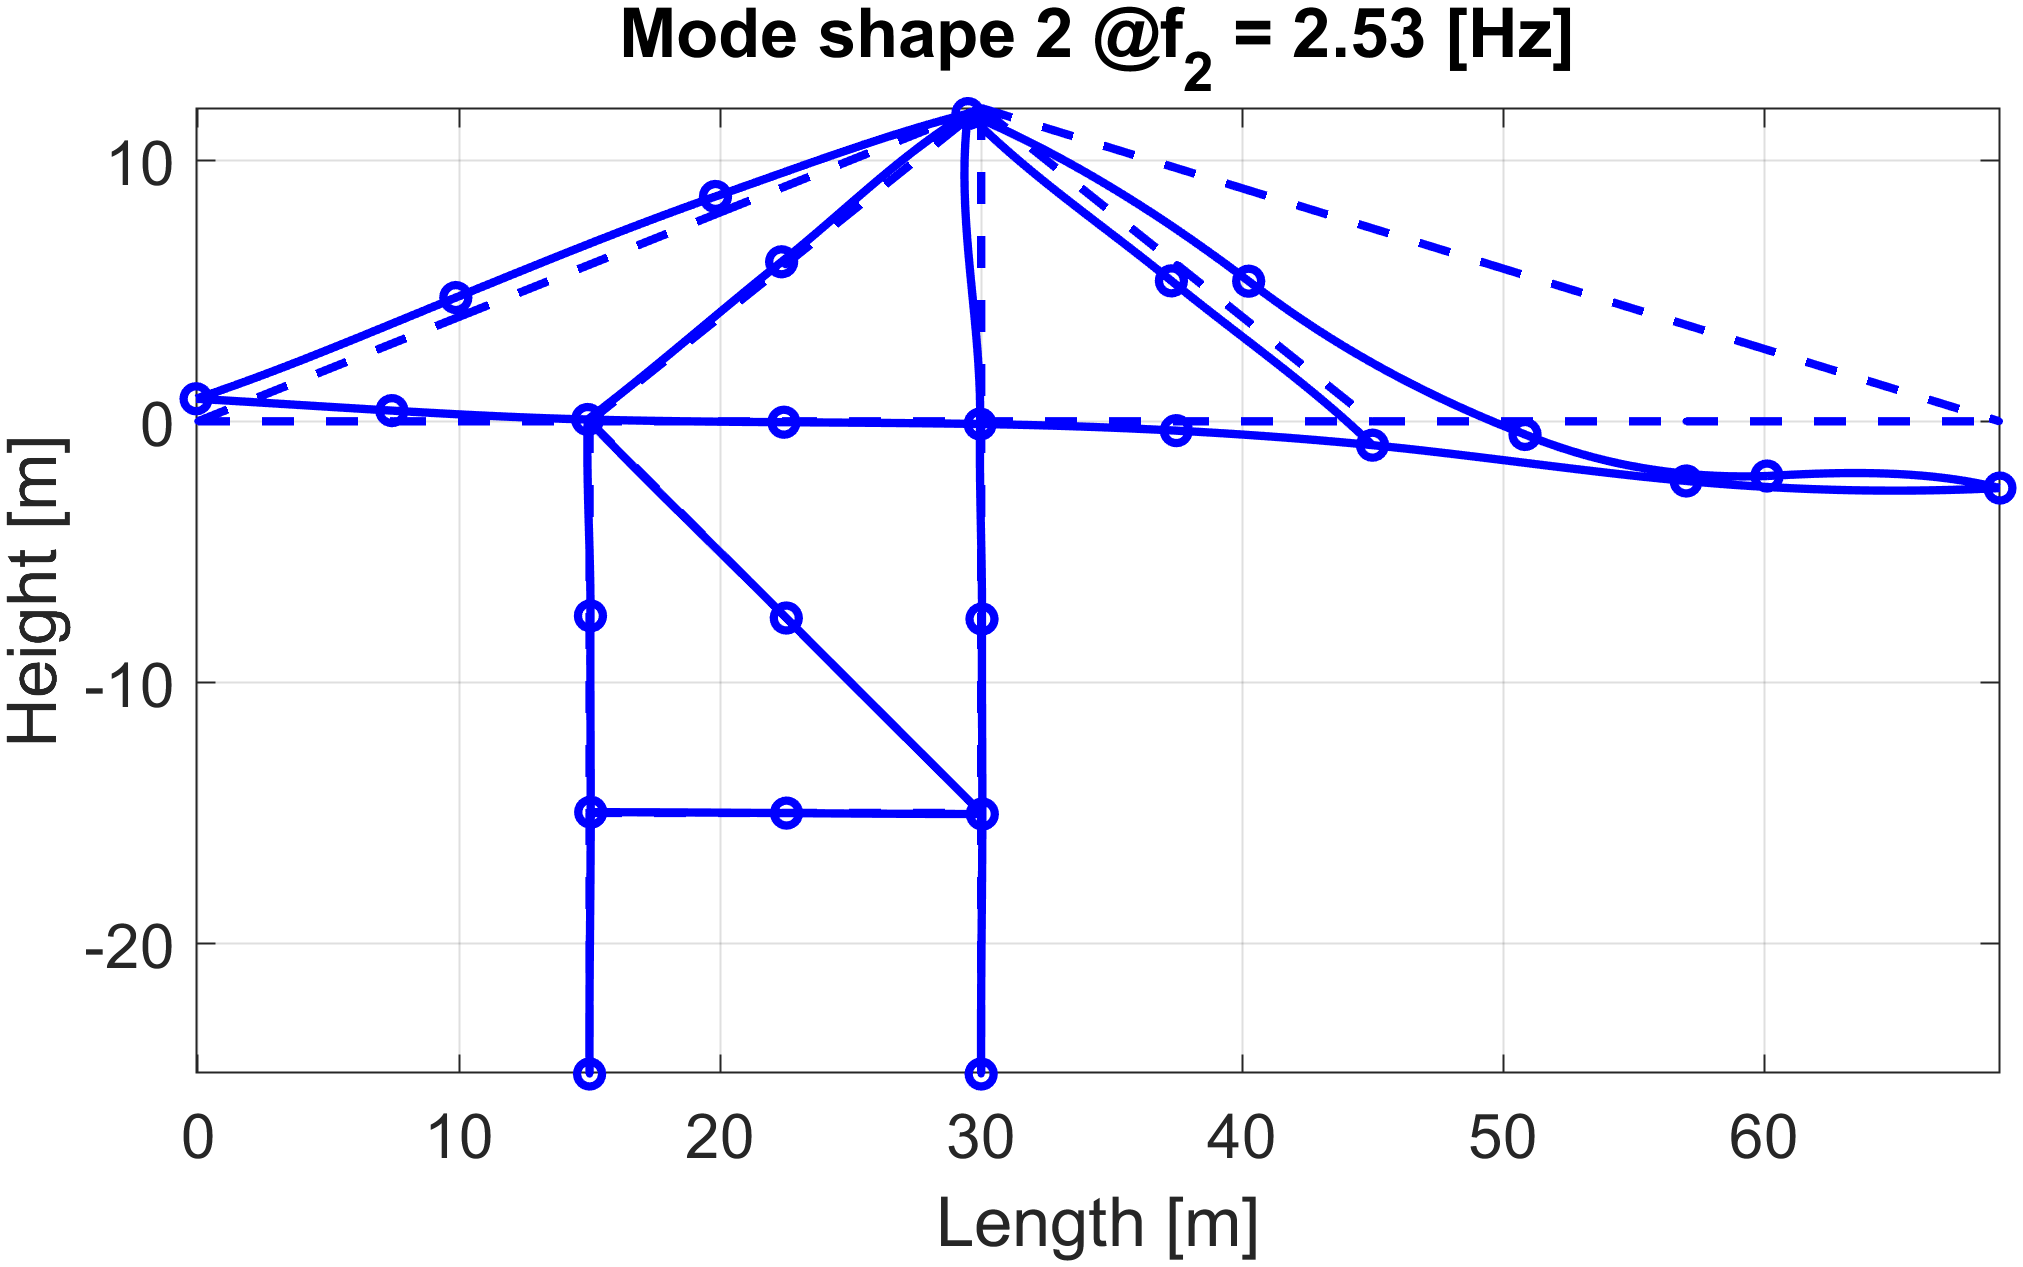
\includegraphics[width=\textwidth]{img/MATLAB/ModeShapes/Mode_02.png}
    \end{minipage}
    \begin{minipage}[b]{0.45\textwidth}
        \centering
        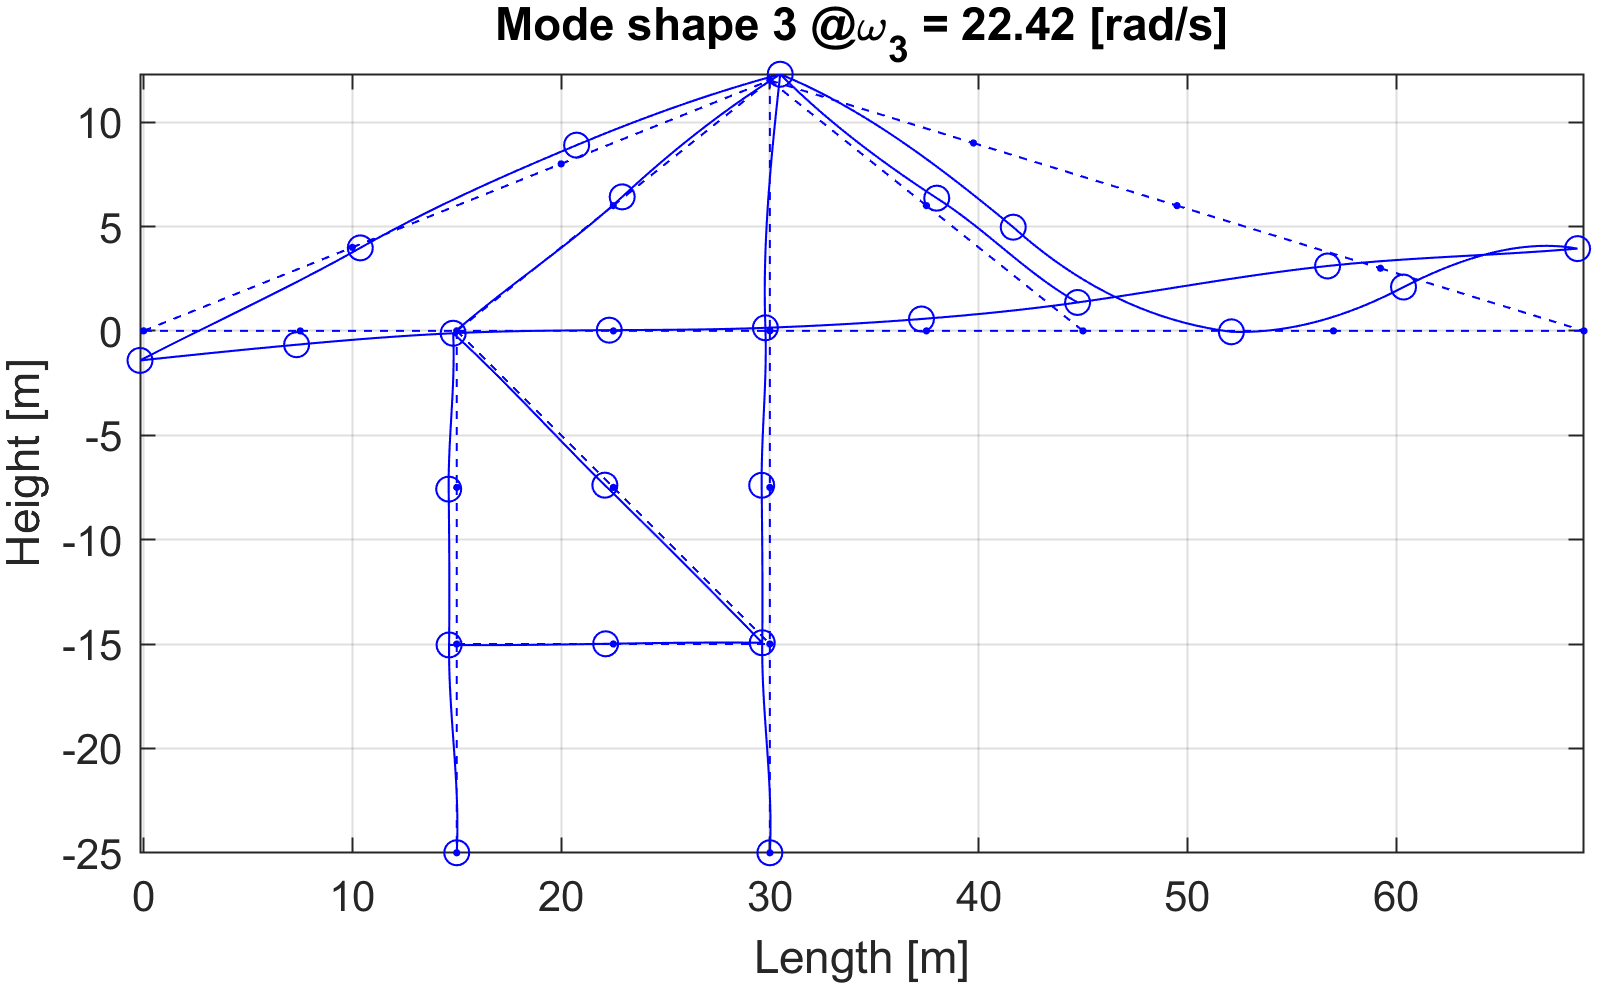
\includegraphics[width=\textwidth]{img/MATLAB/ModeShapes/Mode_03.png}
    \end{minipage}
    \hfill
    \begin{minipage}[b]{0.45\textwidth}
        \centering
        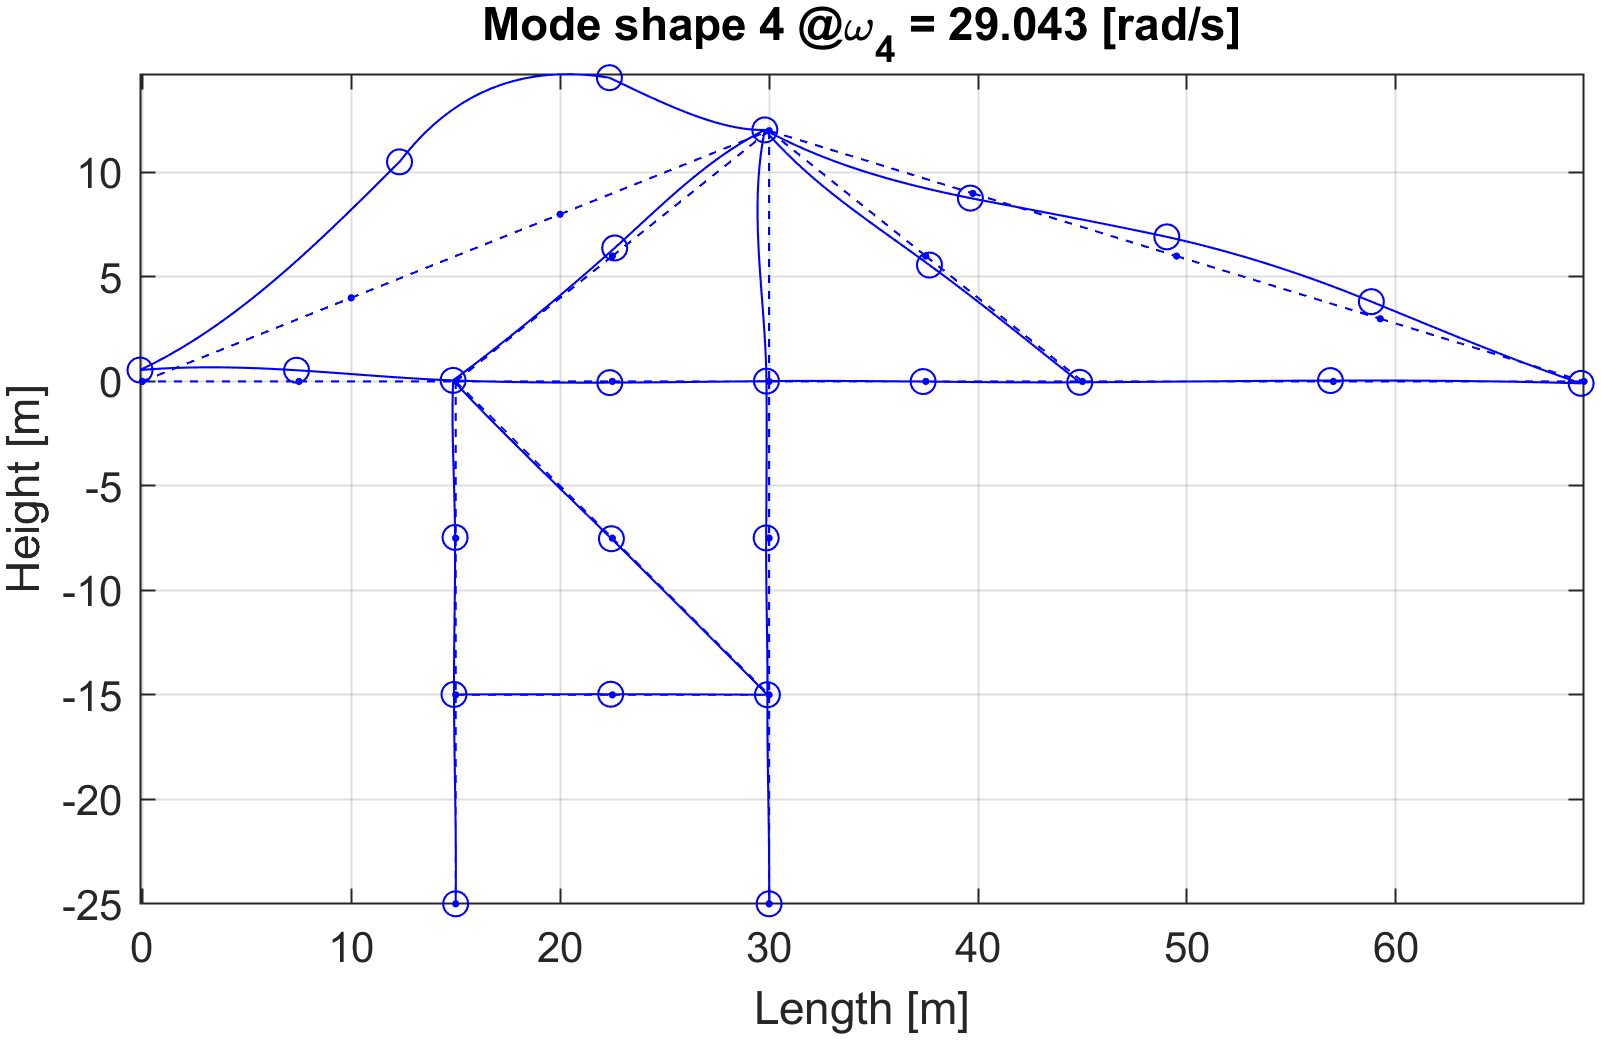
\includegraphics[width=\textwidth]{img/MATLAB/ModeShapes/Mode_04.png}
    \end{minipage}
    \caption{Firsts mode shapes of the FE model}
    \label{fig:mode_shapes}
\end{figure}

\begin{center}
    \huge{The following reasoning is the most interesting of the whole report but must be revised and rewritten in a more straightforward way.}
\end{center}

Notice how the first mode shape is almost a rigid body motion, while the others are more complex and involve bending of the beams.
This can be easily explained by the fact that the equivalent stiffness of the first mode shape is due to only the lateral displacement of the two supporting beam elements that connect the structure to the ground.
This, however, won't be a real problem given that this mode shape is generally not excited by the forces acting on the crane that are usually in the vertical direction.

When we will perform the dynamic analysis of the system, we will see that the mode shapes involved in the response of the system are from the second one on, since they involve the bending of the beams, which is the main source of flexibility of the structure and the one that is directly excited by the vertical forces along the arm of the crane.


\section{FRFs of the structure}
\label{sec:FRFs}

Once the model has been defined and the natural frequencies and mode shapes have been calculated, the next step is to compute the Frequency Response Functions (FRFs) of the structure.
The FRFs are a fundamental tool in the analysis of dynamic systems, as they provide a quantitative measure of the system's response to an external excitation as a function of frequency.

\subsection{FRFs computation}
\label{subsec:FRFs_computation}

To compute the FRFs, we can either use the direct method or the modal superposition method.

\paragraph{Direct method}

The direct method consists of solving the classical equation of motion considering all the degrees of freedom of the system (or equivalently, all the possible mode shapes of the system).

The equation of motion for a linear system can be written as:

\begin{equation}
    \mathbf{M} \ddot{\mathbf{u}} + \mathbf{C} \dot{\mathbf{u}} + \mathbf{K} \mathbf{u} = \mathbf{F}
\end{equation}

Where $\mathbf{M}$, $\mathbf{C}$, and $\mathbf{K}$ are the mass, damping, and stiffness matrices, respectively, $\mathbf{u}$ is the displacement vector, and $\mathbf{F}$ is the external force vector.

To solve this equation, we can work in the complex plane and then consider the real part of the solution to obtain the physical response of the system.

By doing so, the FRF can be computed as:

\begin{equation}
    \mathbf{H}(j\omega) = (-\omega^2 \mathbf{M} + j\omega \mathbf{C} + \mathbf{K})^{-1} \mathbf{F}
\end{equation}

Where $\mathbf{H}(j\omega)$ is the FRF relating the particular set of forces $\mathbf{F}$ applied in one or more nodes, to the response of any other node of the structure.

In \texttt{MATLAB}, the FRFs based on direct approach can be implemented as follows:

\begin{lstlisting}[language=Matlab]

    % Here we compute the FRFs due to a vertical force applied to node A with module 1
    F_F(node_A_vertical) = 1;

    FRF_direct_approach = zeros(size(M_FF, 1), length(omega_vet));
    for ii = 1:length(omega_vet)
        FRF_direct_approach(:, ii) = (-omega_vet(ii)^2 * M_FF + 1i*omega_vet(ii) * C_FF + K_FF) \ F_F;
    end

\end{lstlisting}


\paragraph{Modal superposition method}

The modal superposition method is an alternative approach to compute the FRFs of a structure.
It is based on the modal decomposition of the system response, which allows us to reduce the number of degrees of freedom to consider.

The idea behind this approach, is to consider as negligible the contribution of the higher modes of the system, and to focus only on the first few modes that are significant in the frequency range of interest.

Having this hypothesis in mind, we can proceed with the orthogonalization of the global matrices based on the first $n$ mode shapes of the system, which indeed a significant reduction in size of the given problem.
As an example, if we consider the first $n=5$ mode shapes of the system, all the matrices will be reduced to a $5 \times 5$ size, and FRFs matrix will also be reduced to a $5 \times size(\omega_{vector})$.

This approach, in general, is more efficient than the direct method, especially when the number of degrees of freedom of the system is high.
However, as we can imagine, the accuracy of the results will strongly depend on the number of modes considered in the analysis and the position of the forces acting on the structure.

In \texttt{MATLAB}, the FRFs based on modal superposition can be implemented as follows:

\begin{lstlisting}[language=Matlab]

    % To observe the approximation introduced, we consider only 2 modes
    % Here we compute the FRFs due to a vertical force applied to node A with module 1

    F_F(node_A_vertical) = 1;

    Phi_reduced = mode_shapes(:, 1:2);
    M_FF_modal_reduced = Phi_reduced' * M_FF * Phi_reduced;
    C_FF_modal_reduced = Phi_reduced' * C_FF * Phi_reduced;
    K_FF_modal_reduced = Phi_reduced' * K_FF * Phi_reduced;
    F_F_modal = Phi_reduced' * F_F;

    FRF_modal_approach = zeros(size(M_FF_modal_reduced, 1), length(omega_vet));
    for ii = 1:length(omega_vet)
        FRF_modal_approach(:, ii) = (-omega_vet(ii)^2 * M_FF_modal_reduced + 1i*omega_vet(ii) * C_FF_modal_reduced + K_FF_modal_reduced) \ F_F_modal;
    end

    FRF_modal_approach = Phi_reduced * FRF_modal_approach;

\end{lstlisting}

Notice that, even if the size of the FRFs matrix is reduced, the final result must be projected back to the original space to obtain the physical response of the system.

The transformation between on set of coordinates and the other is done via the matrix $[\Phi]$ composed by the mode shapes of the system (in this case, the first $n$ mode shapes).

\subsection{FRFs examples}
\label{subsec:FRFs_examples}

In this section we will show some examples of FRFs computed for the harbour crane model, and, for some of them, we will discuss the results obtained using both the direct method and the modal superposition method.

\subsubsection{Direct method - Vertical force \textbf{A} to Vertical displacement \textbf{A} and Horizontal displacement \textbf{B}}
\label{subsubsec:direct_method_vertical_force_A}

In this example, we compute the FRF relating the vertical displacement of node \textbf{A} and the horizontal displacement of node \textbf{B} to the vertical force applied to node \textbf{A}.
The FRFs are computed using the direct method, considering all the degrees of freedom of the system.

\begin{figure}[H]
    \centering
    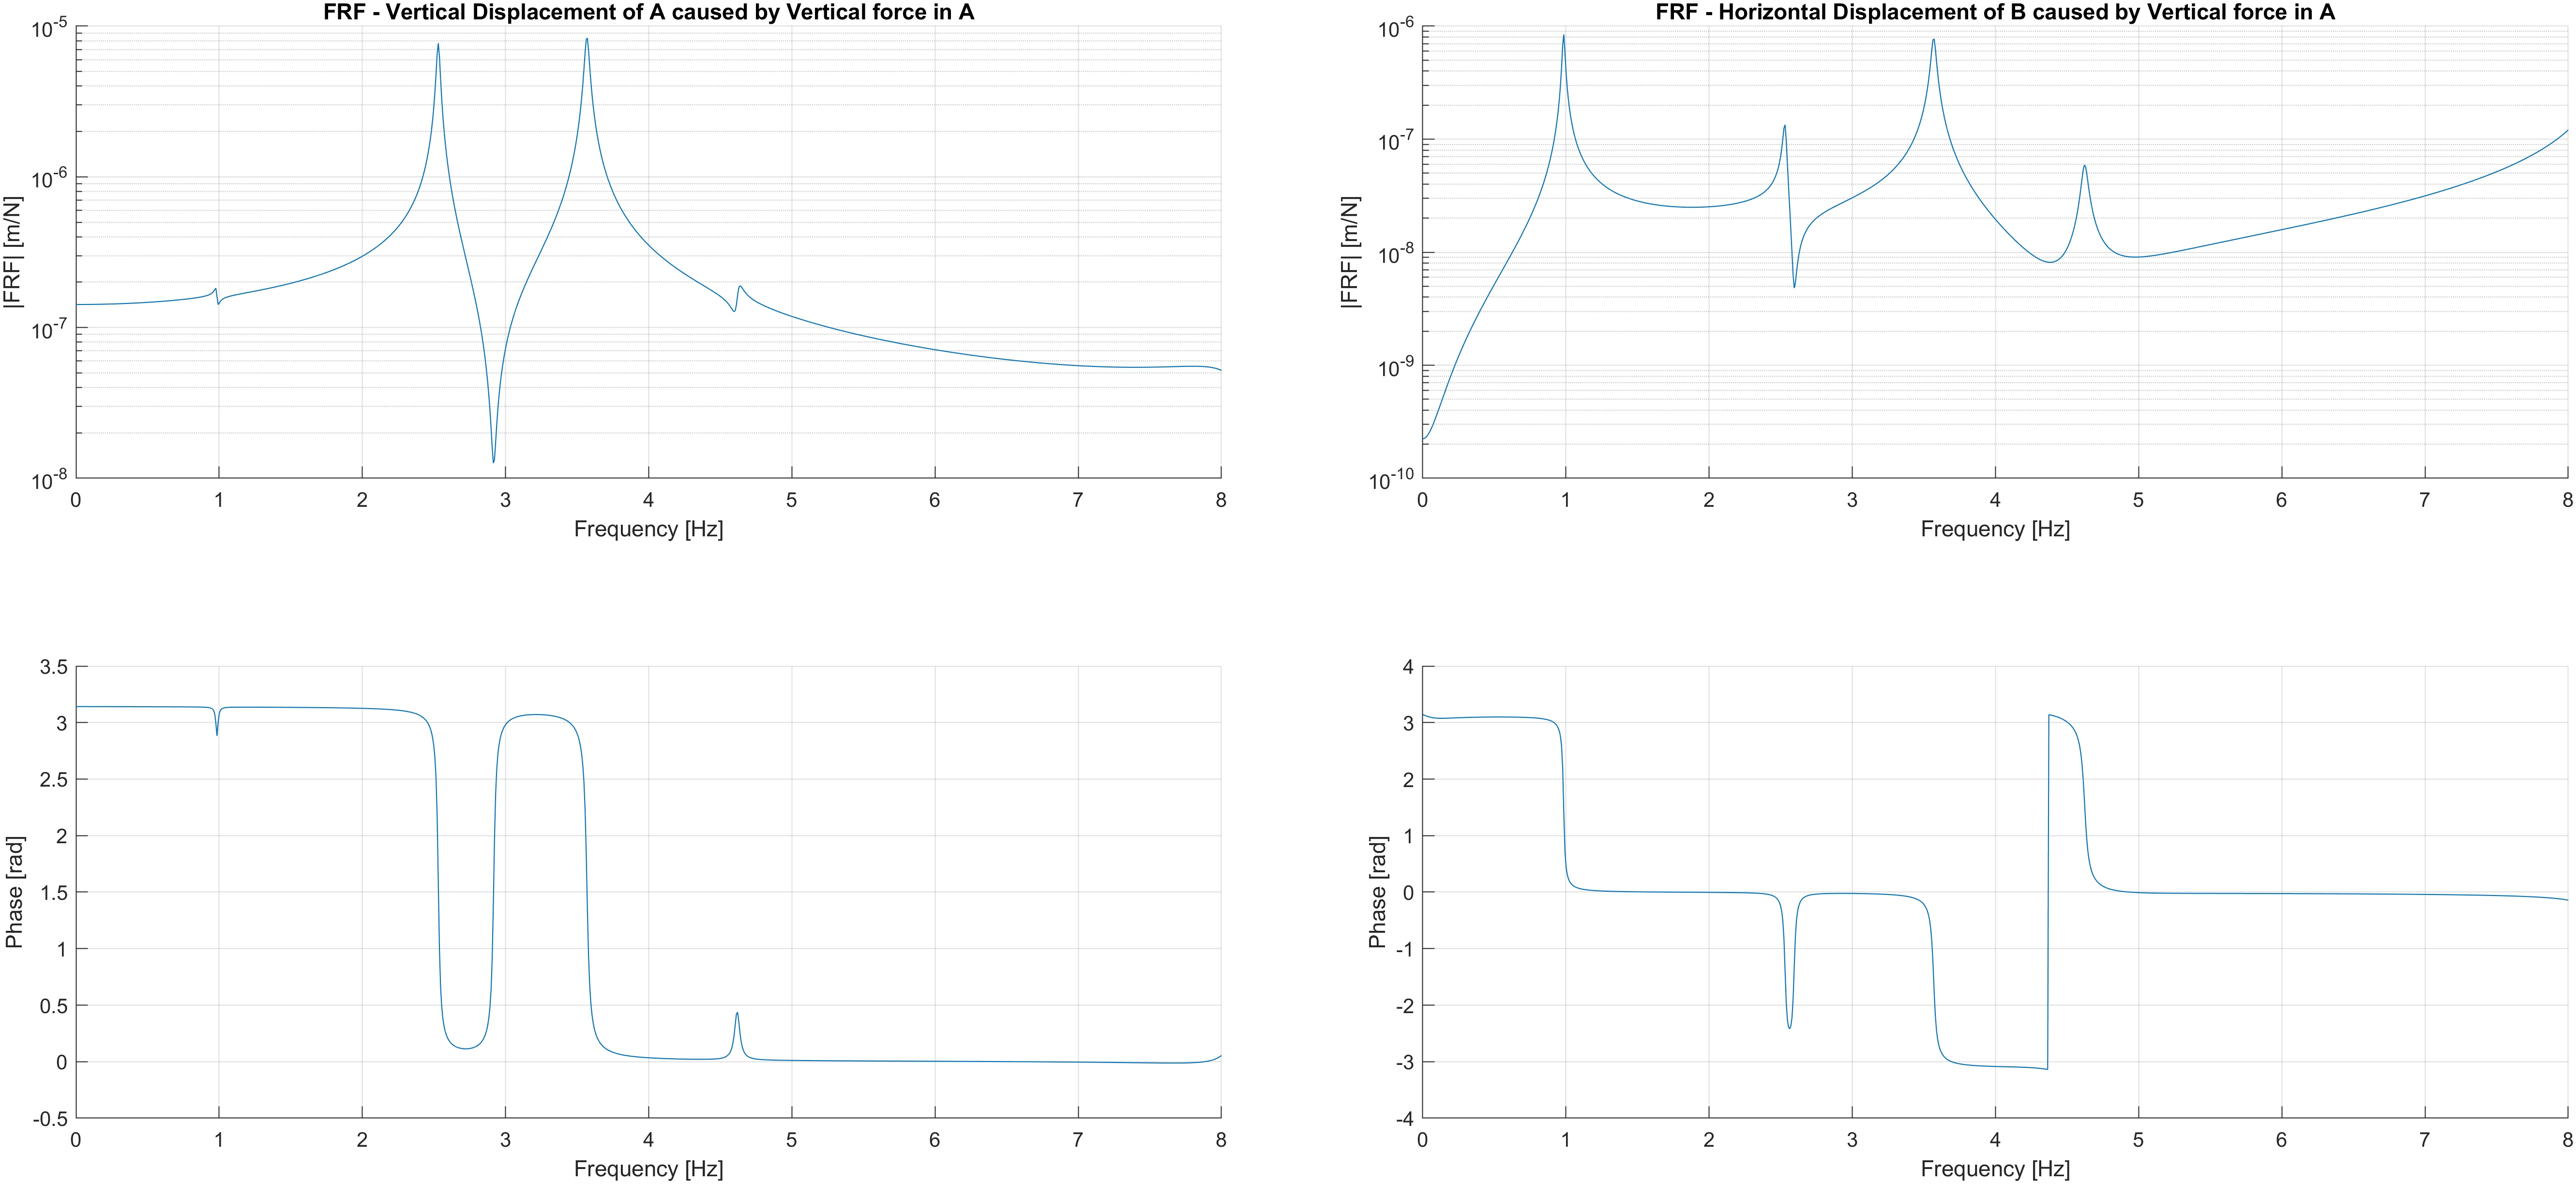
\includegraphics[width=\textwidth]{img/MATLAB/FRFs/Vertical_in_A.png}
    \caption{FRF computed using the direct method - Vertical force \textbf{A} to Vertical displacement \textbf{A} and Horizontal displacement \textbf{B}.}
    \label{fig:FRF_direct_vertical_A}
\end{figure}

From the FRFs shown in Figure \ref{fig:FRF_direct_vertical_A}, we can observe that in the considered frequency range ($0-8 [Hz]$), the vertical displacement of node \textbf{A} is more sensitive to the vertical force applied to node \textbf{A} than the horizontal displacement of node \textbf{B}.

Moreover, as expected, the resonance peaks in the FRFs correspond to the natural frequencies of the system found during modal analysis (see Section \ref{sub:modal_analysis}).

Interestingly, both FRFs exhibit an anti-resonance peak between the third and fourth natural frequencies (at $\approx 2.91 [Hz] \rightarrow 18.28 [rad/s]$), which indicates that the system's response to the excitation is minimized at that frequency.
In other words, at that specific excitation frequency, node \textbf{A} became stationary and any force applied at the corresponding frequency will not excite the system (no energy can flow from the force to the structure, null virtual work).


\subsubsection{Direct vs. Modal superposition method - Vertical force \textbf{A} to Horizontal displacement B}
\label{subsubsec:direct_vs_modal_vertical_force_A}

In this example, we compute the FRF relating the horizontal displacement of node \textbf{B} to the vertical force applied to node \textbf{A}.
We compare the results obtained using the direct method and the modal superposition method.

In order to have a significant comparison of the effect of the reduction of the number of modes considered in the analysis, we will consider only the first two mode shapes of the system in the modal superposition method ($n=2$).

\begin{figure}[H]
    \centering
    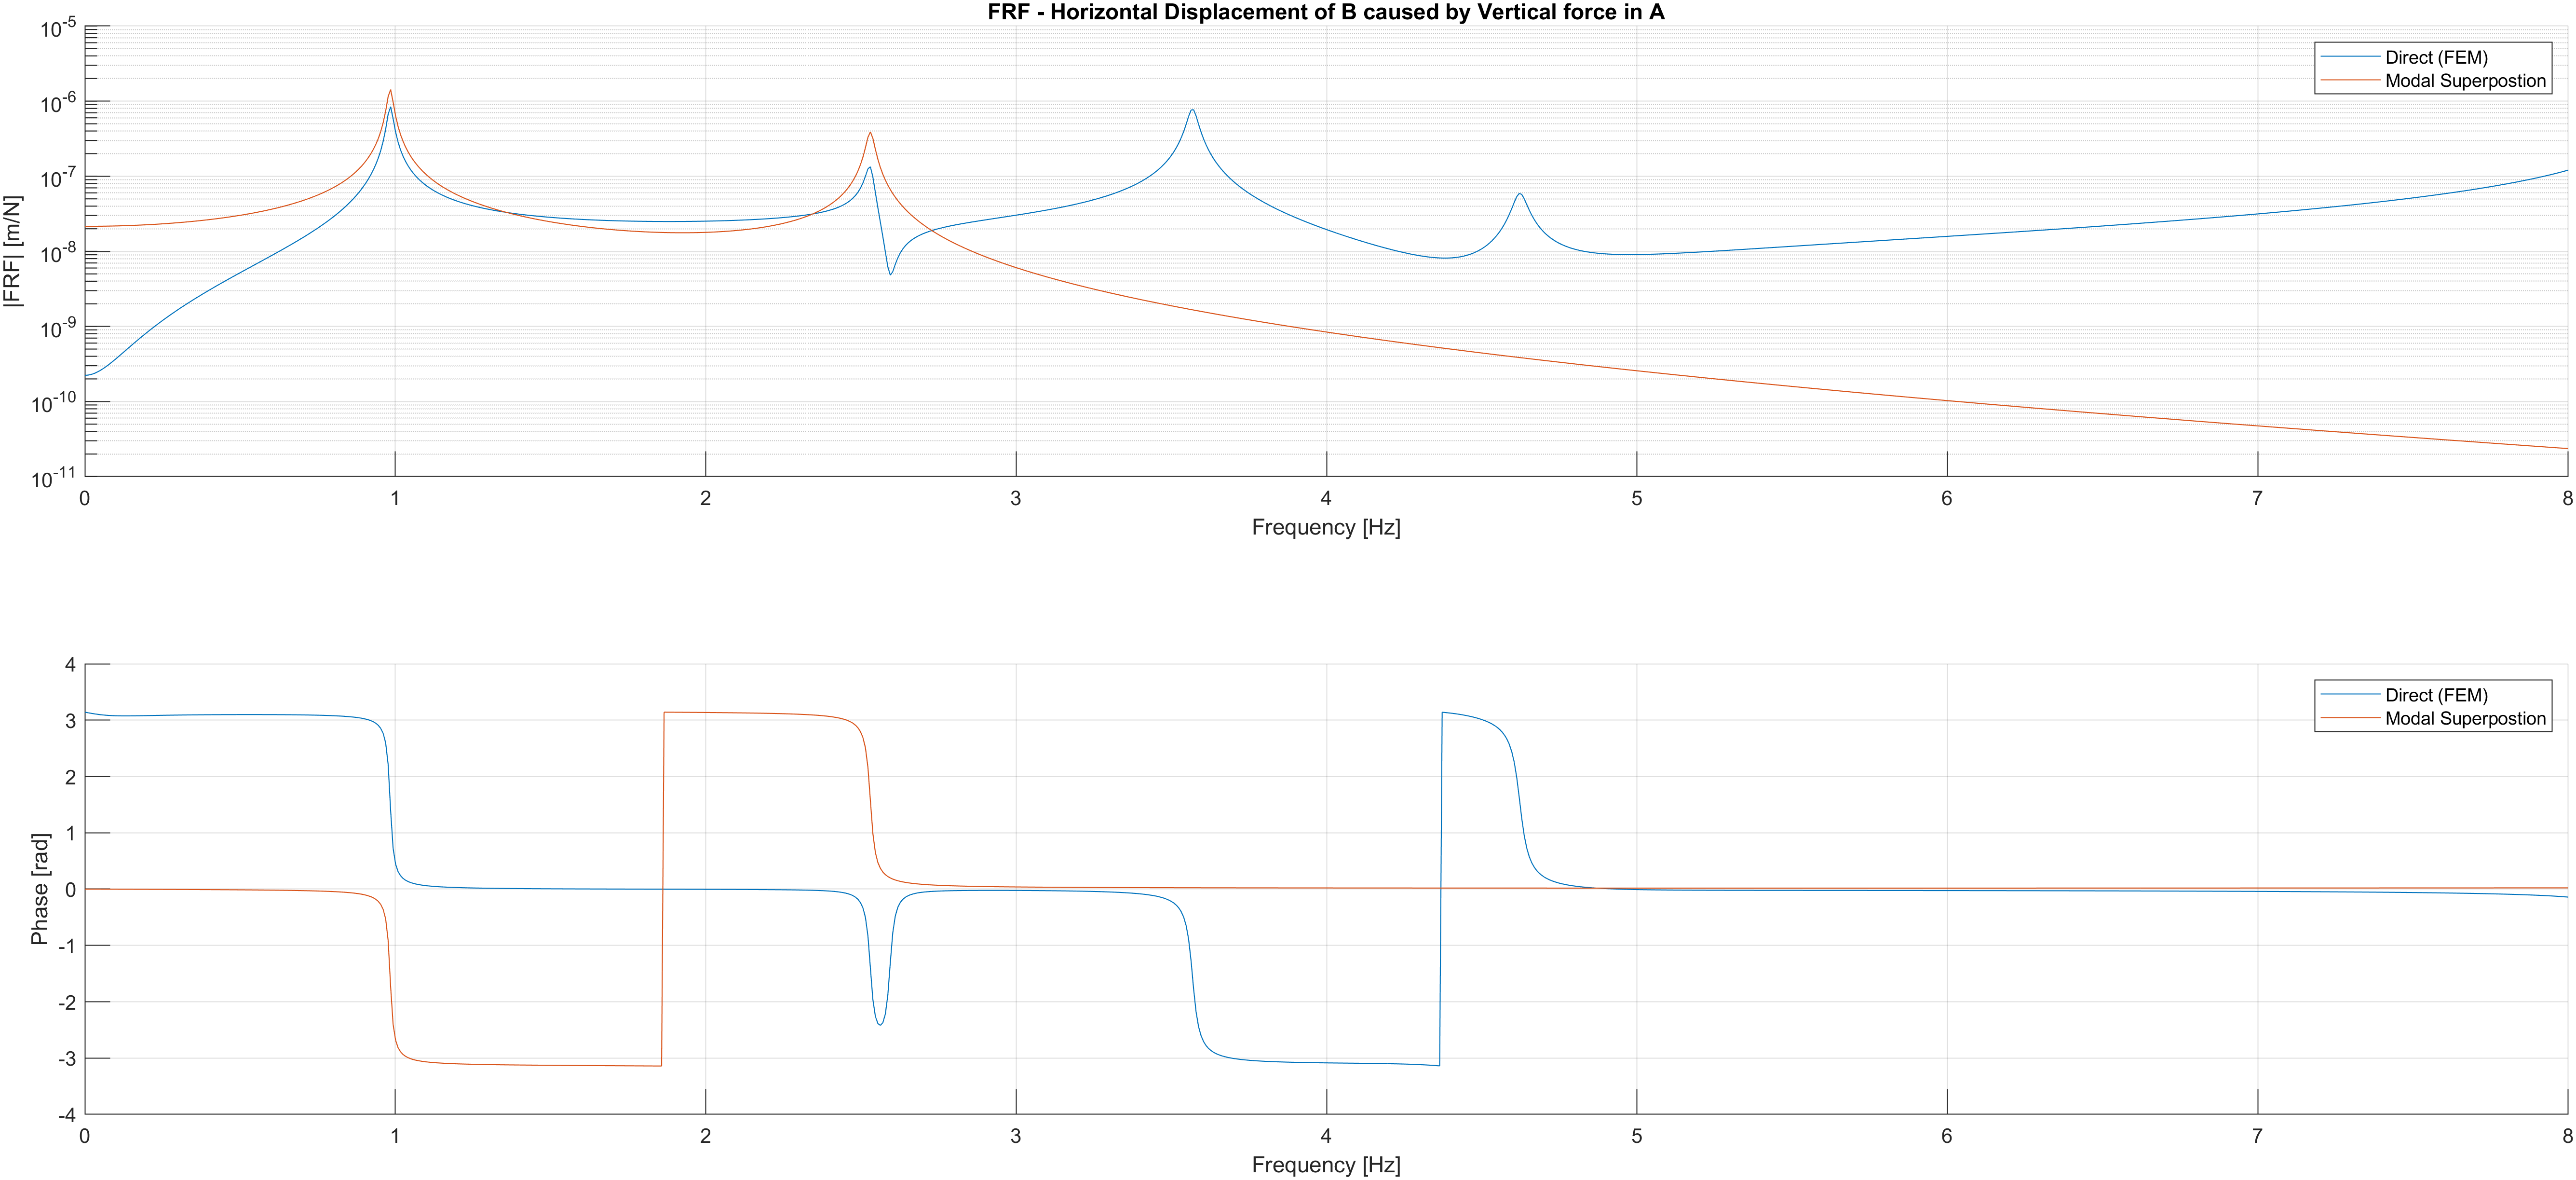
\includegraphics[width=\textwidth]{img/MATLAB/FRFs/Direct_vs_Modal.png}
    \caption{FRF computed using the direct method and modal superposition method - Vertical force \textbf{A} to Horizontal displacement \textbf{B}.}
    \label{fig:FRF_direct_vs_modal_vertical_A}
\end{figure}

From the FRFs shown in Figure \ref{fig:FRF_direct_vs_modal_vertical_A}, we can observe that the results obtained using the direct method and the modal superposition method are in good agreement only around the considered natural frequencies of the system.
As we move away from the peaks, the results start to diverge.

This behavior is expected since the modal superposition method considers only the first two mode shapes of the system, which may not capture the full dynamic behavior of the structure.
On the other hand, the direct method considers all the degrees of freedom of the system, providing a more accurate representation of the system's response to the excitation (at the cost of higher computational effort).


\subsubsection{Direct method - Vertical force \textbf{C} to Vertical reaction force \textbf{O2}}
\label{subsubsec:direct_method_vertical_force_C}

In this example, we compute the FRF relating the vertical reaction force at node \textbf{O2} to the vertical force applied to node \textbf{C}.
The FRF is computed using the direct method, considering all the degrees of freedom of the system.

\begin{figure}[H]
    \centering
    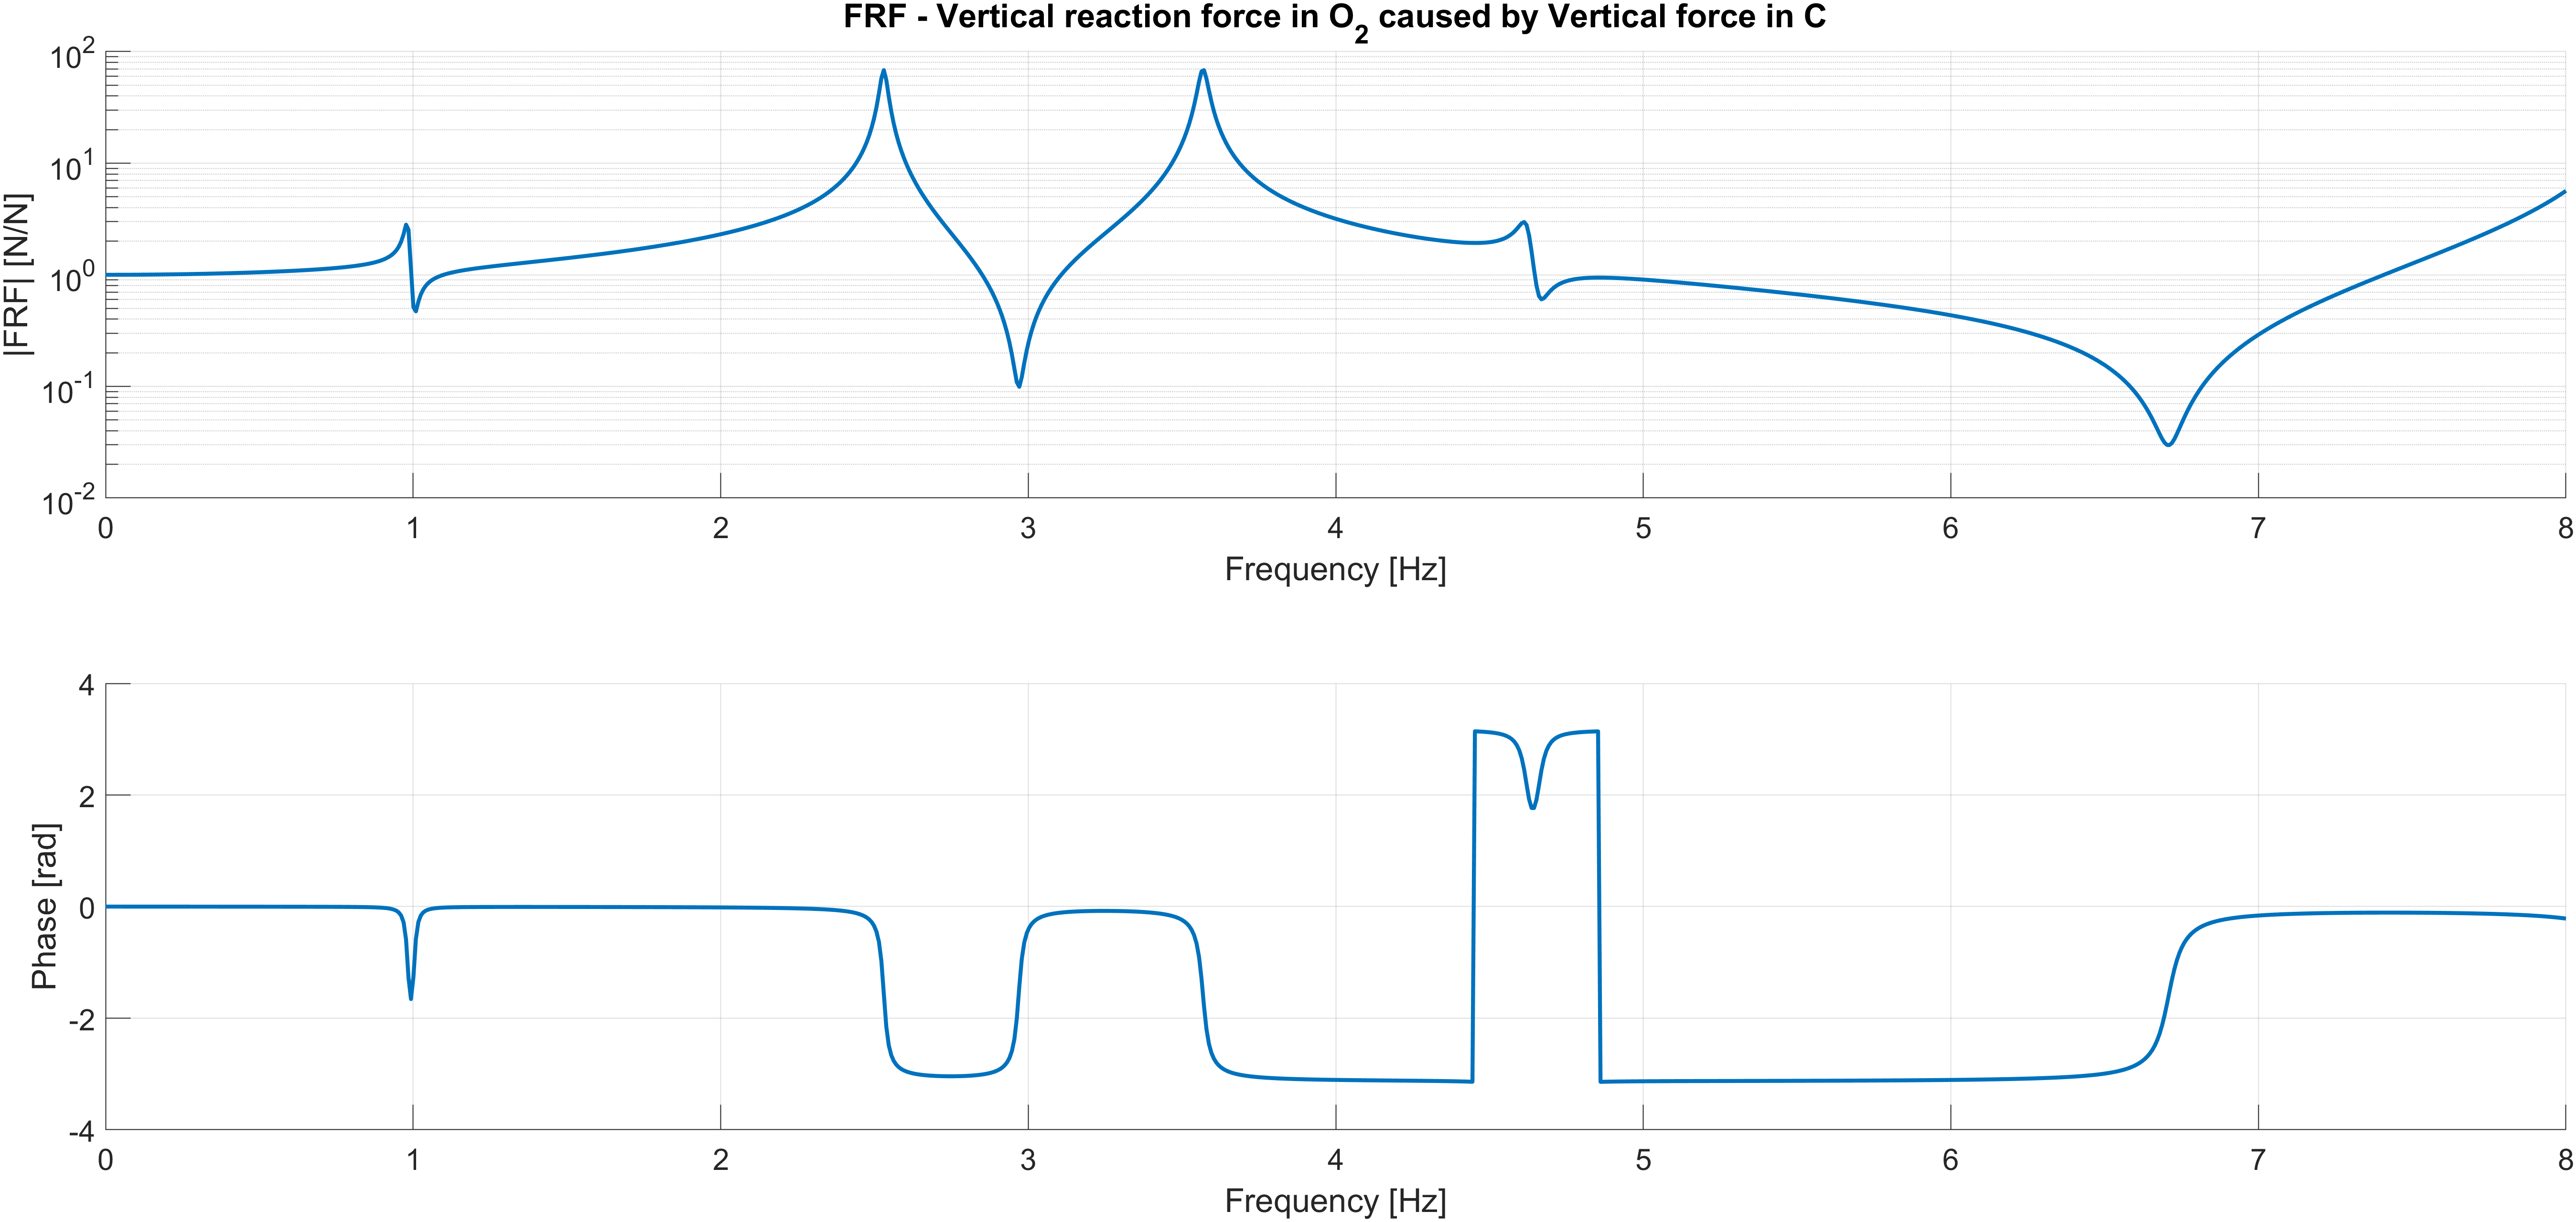
\includegraphics[width=\textwidth]{img/MATLAB/FRFs/Reaction_O2.png}
    \caption{FRF computed using the direct method - Vertical force \textbf{C} to Vertical reaction force \textbf{O2}}
    \label{fig:FRF_direct_vertical_C}
\end{figure}

Notice that reaction forces are computed in two consecutive steps: first, using the direct method the displacement in time of each node is computed obtaining the vector $\mathbf{q}(t)$, then the reaction forces are computed by substituting the displacement vector in the equation of motion relative to the constrained nodes, obtaining the reaction forces vector $\mathbf{R}(t)$.
\section{Static responses of the structure}
\label{sec:static_responses}

In this section, the static responses of the structure are computed.
The static responses are the displacements of the structure when subjected to a static load.

Again, as in many other engineering problems, we can approach this problem in at least a couple of different ways.
In the following, we will explain how to compute the static responses of the structure using both a displacement approach and an acceleration approach.

Notice that the two method differs only in the way the global force vector $\mathbf{F}$ is assembled.
In the end, once $\mathbf{F}$ is known, both methods will solve the steady state version of the equation of motion:

\begin{equation}
    \mathbf{K} \mathbf{u} = \mathbf{F}
    \label{eq:static_responses}
\end{equation}

Where $\mathbf{K}$ is the stiffness matrix of the structure, $\mathbf{u}$ is the vector of displacements and $\mathbf{F}$ is the global force vector.

\subsection{Displacement approach}
\label{subsec:displacement_approach}

The displacement approach consists of assembling the global force vector $\mathbf{F_F}$ based on the `displacement method' used in structural mechanics.

In particular, if the structure is subjected to a distributed static load (as in the case of the gravity load), we know that the nodal forces on a single beam element can be computed as:

\begin{figure}[H]
    \centering
    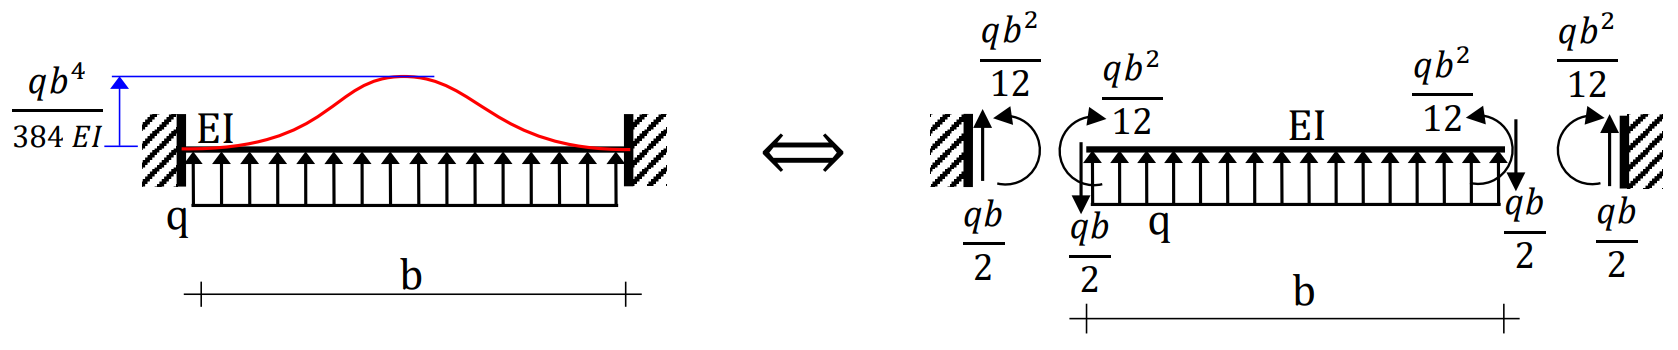
\includegraphics[width=0.9\textwidth]{img/displacement-method.png}
    \caption{Displacement method for distributed loads.}
    \label{fig:displacement_method}
\end{figure}

From the figure above, we can obtain the coefficients needed to compute the equivalent nodal forces due to a distributed load along the element.

By using proper change in the reference system (by rotational matrices), it's possible to build the equivalent global force vector $\mathbf{F_F}$, which can be seen as the equivalent effect on the node of the structure due to the distributed load.

Finally, we can solve the equation of motion \ref{eq:static_responses} to obtain the displacements of the structure.

In \texttt{MATLAB}, the displacement approach can be implemented as follows:

\begin{lstlisting}[language=Matlab, caption={Displacement approach to compute the static responses of the structure.}]
    % Displacement approach.
    F_F_global = zeros(3*nnod, 1);

    for ii = 1:nbeam

        [R, Q] = compute_rotational_matrices(gamma(ii));

        % Here we are negletting the possibility of a distributed momentum
        % load. Just distributed force loads are considered.
        elemental_distributed_load = R(1:2, 1:2)' * [0 -9.81 * m(ii)]';

        elemental_equivalent_nodal_load = [
            l(ii)/2 0
            0       l(ii)/2
            0       l(ii)^2/12
            l(ii)/2 0
            0       l(ii)/2
            0       -l(ii)^2/12
            ] * elemental_distributed_load;

        global_equivalent_nodal_load = Q * elemental_equivalent_nodal_load;

        F_F_global(incid(ii, :)) = F_F_global(incid(ii, :)) + global_equivalent_nodal_load;

    end

    X_gravity_displacement_approach = K_FF \ F_F_global(1:ndof);
\end{lstlisting}
\subsection{Acceleration approach}
\label{subsec:acceleration_approach}

The acceleration approach instead, consists of assembling the global force vector $\mathbf{F_F}$ based on the idea that the structure (since it has been discretized), can be seen as a system of masses connected by springs and dampers.
Because of this, a distributed acceleration load can be directly transformed into a series of nodal forces by solving the second Newton's law for each node of the structure.

In particular, the nodal forces can be computed as:

\begin{equation}
    \mathbf{F_F} = [M_{FF}] \cdot \mathbf{a}
\end{equation}

Where $[M_{FF}]$ is the mass matrix of the structure and $\mathbf{a}$ is the vector of accelerations acting on each degree of freedom of the structure.

Finally, we can solve the equation of motion \ref{eq:static_responses} to obtain the displacements of the structure.

In \texttt{MATLAB}, the acceleration approach can be implemented as follows:

\begin{lstlisting}[language=Matlab, caption={Acceleration approach to compute the static responses of the structure.}]
    % Acceleration approach.
    x_dot_dot = zeros(ndof, 1);
    x_dot_dot(idb(:, 2)) = -9.81;

    F_F_nodal = M * x_dot_dot;

    X_gravity_acceleration_approach = K_FF \ F_F_nodal(1:ndof);
\end{lstlisting}

\subsection{Comparison of the two methods}
\label{subsec:comparison_of_the_two_methods}

As we can see from Figure \ref{fig:static_responses}, the two methods give the same results.
This is expected given that the acceleration approach is just a derivation of the displacement approach, since the mass matrices $M$ and the stiffness matrices $K$ are just an implementation of the displacement and/or the force method used to solve structures.

\begin{figure}[H]
    \centering
    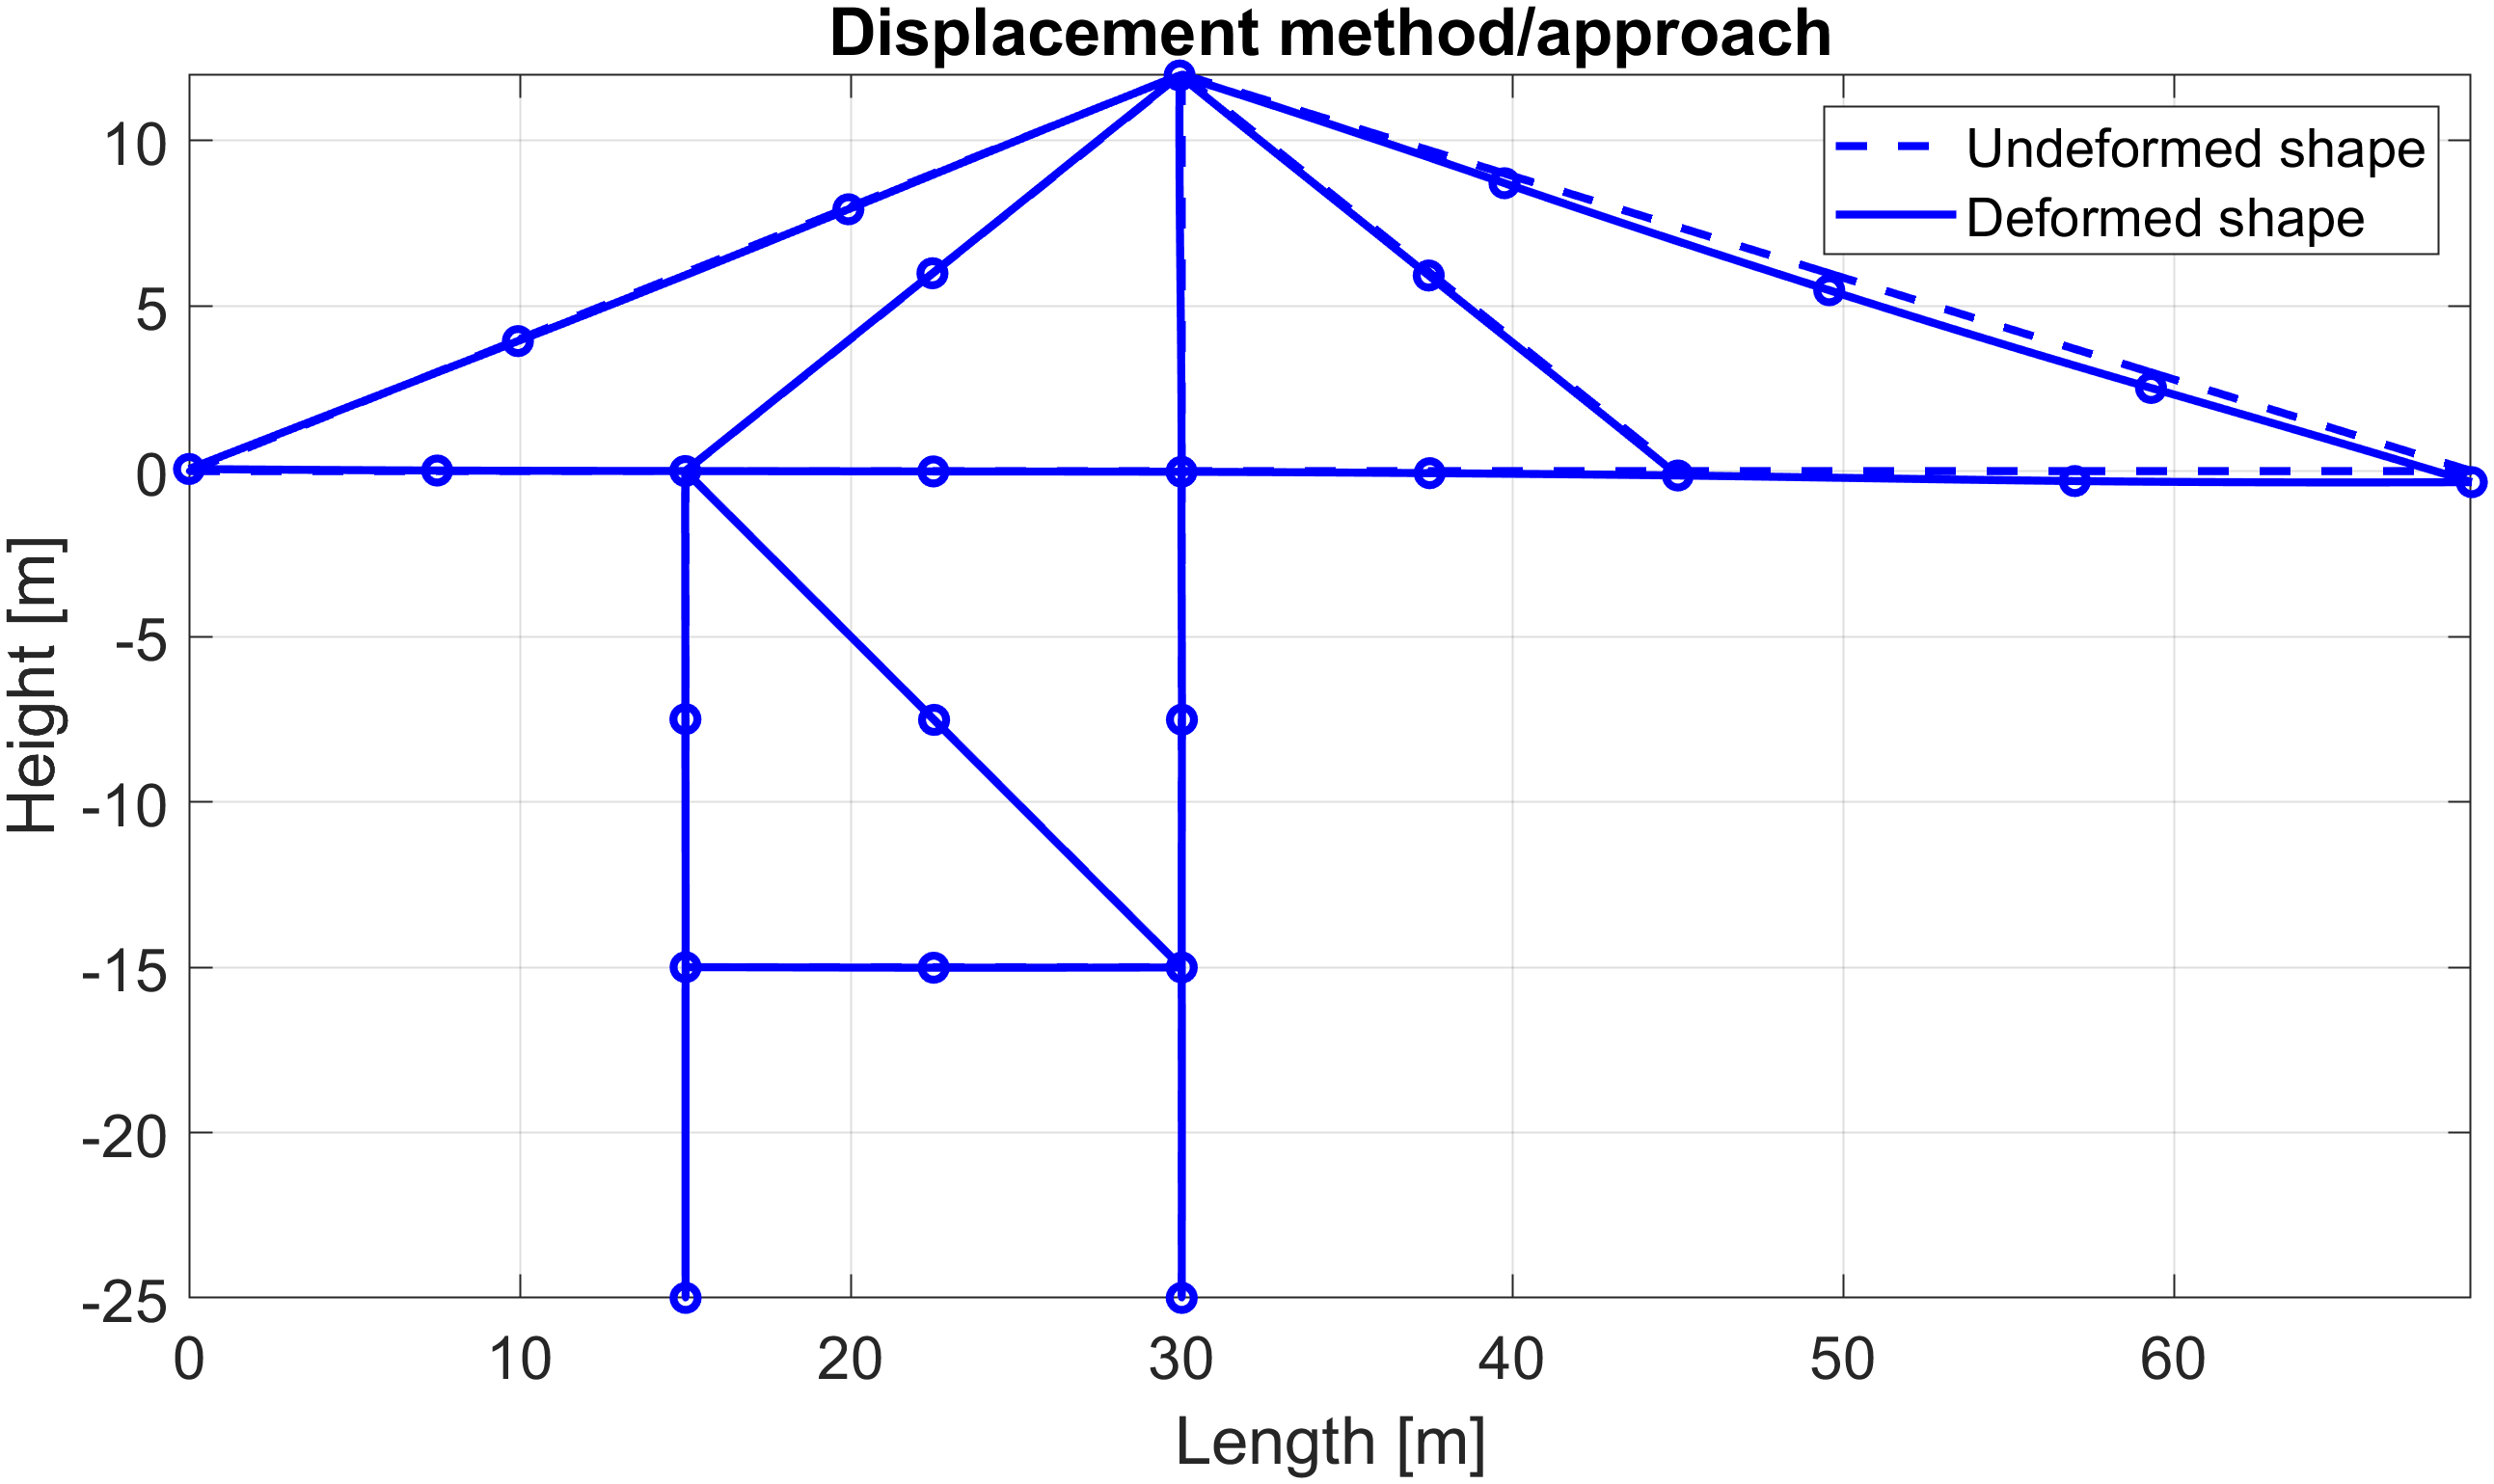
\includegraphics[width=0.45\textwidth]{img/MATLAB/Responses/Gravity_displacement.png}
    \hfill
    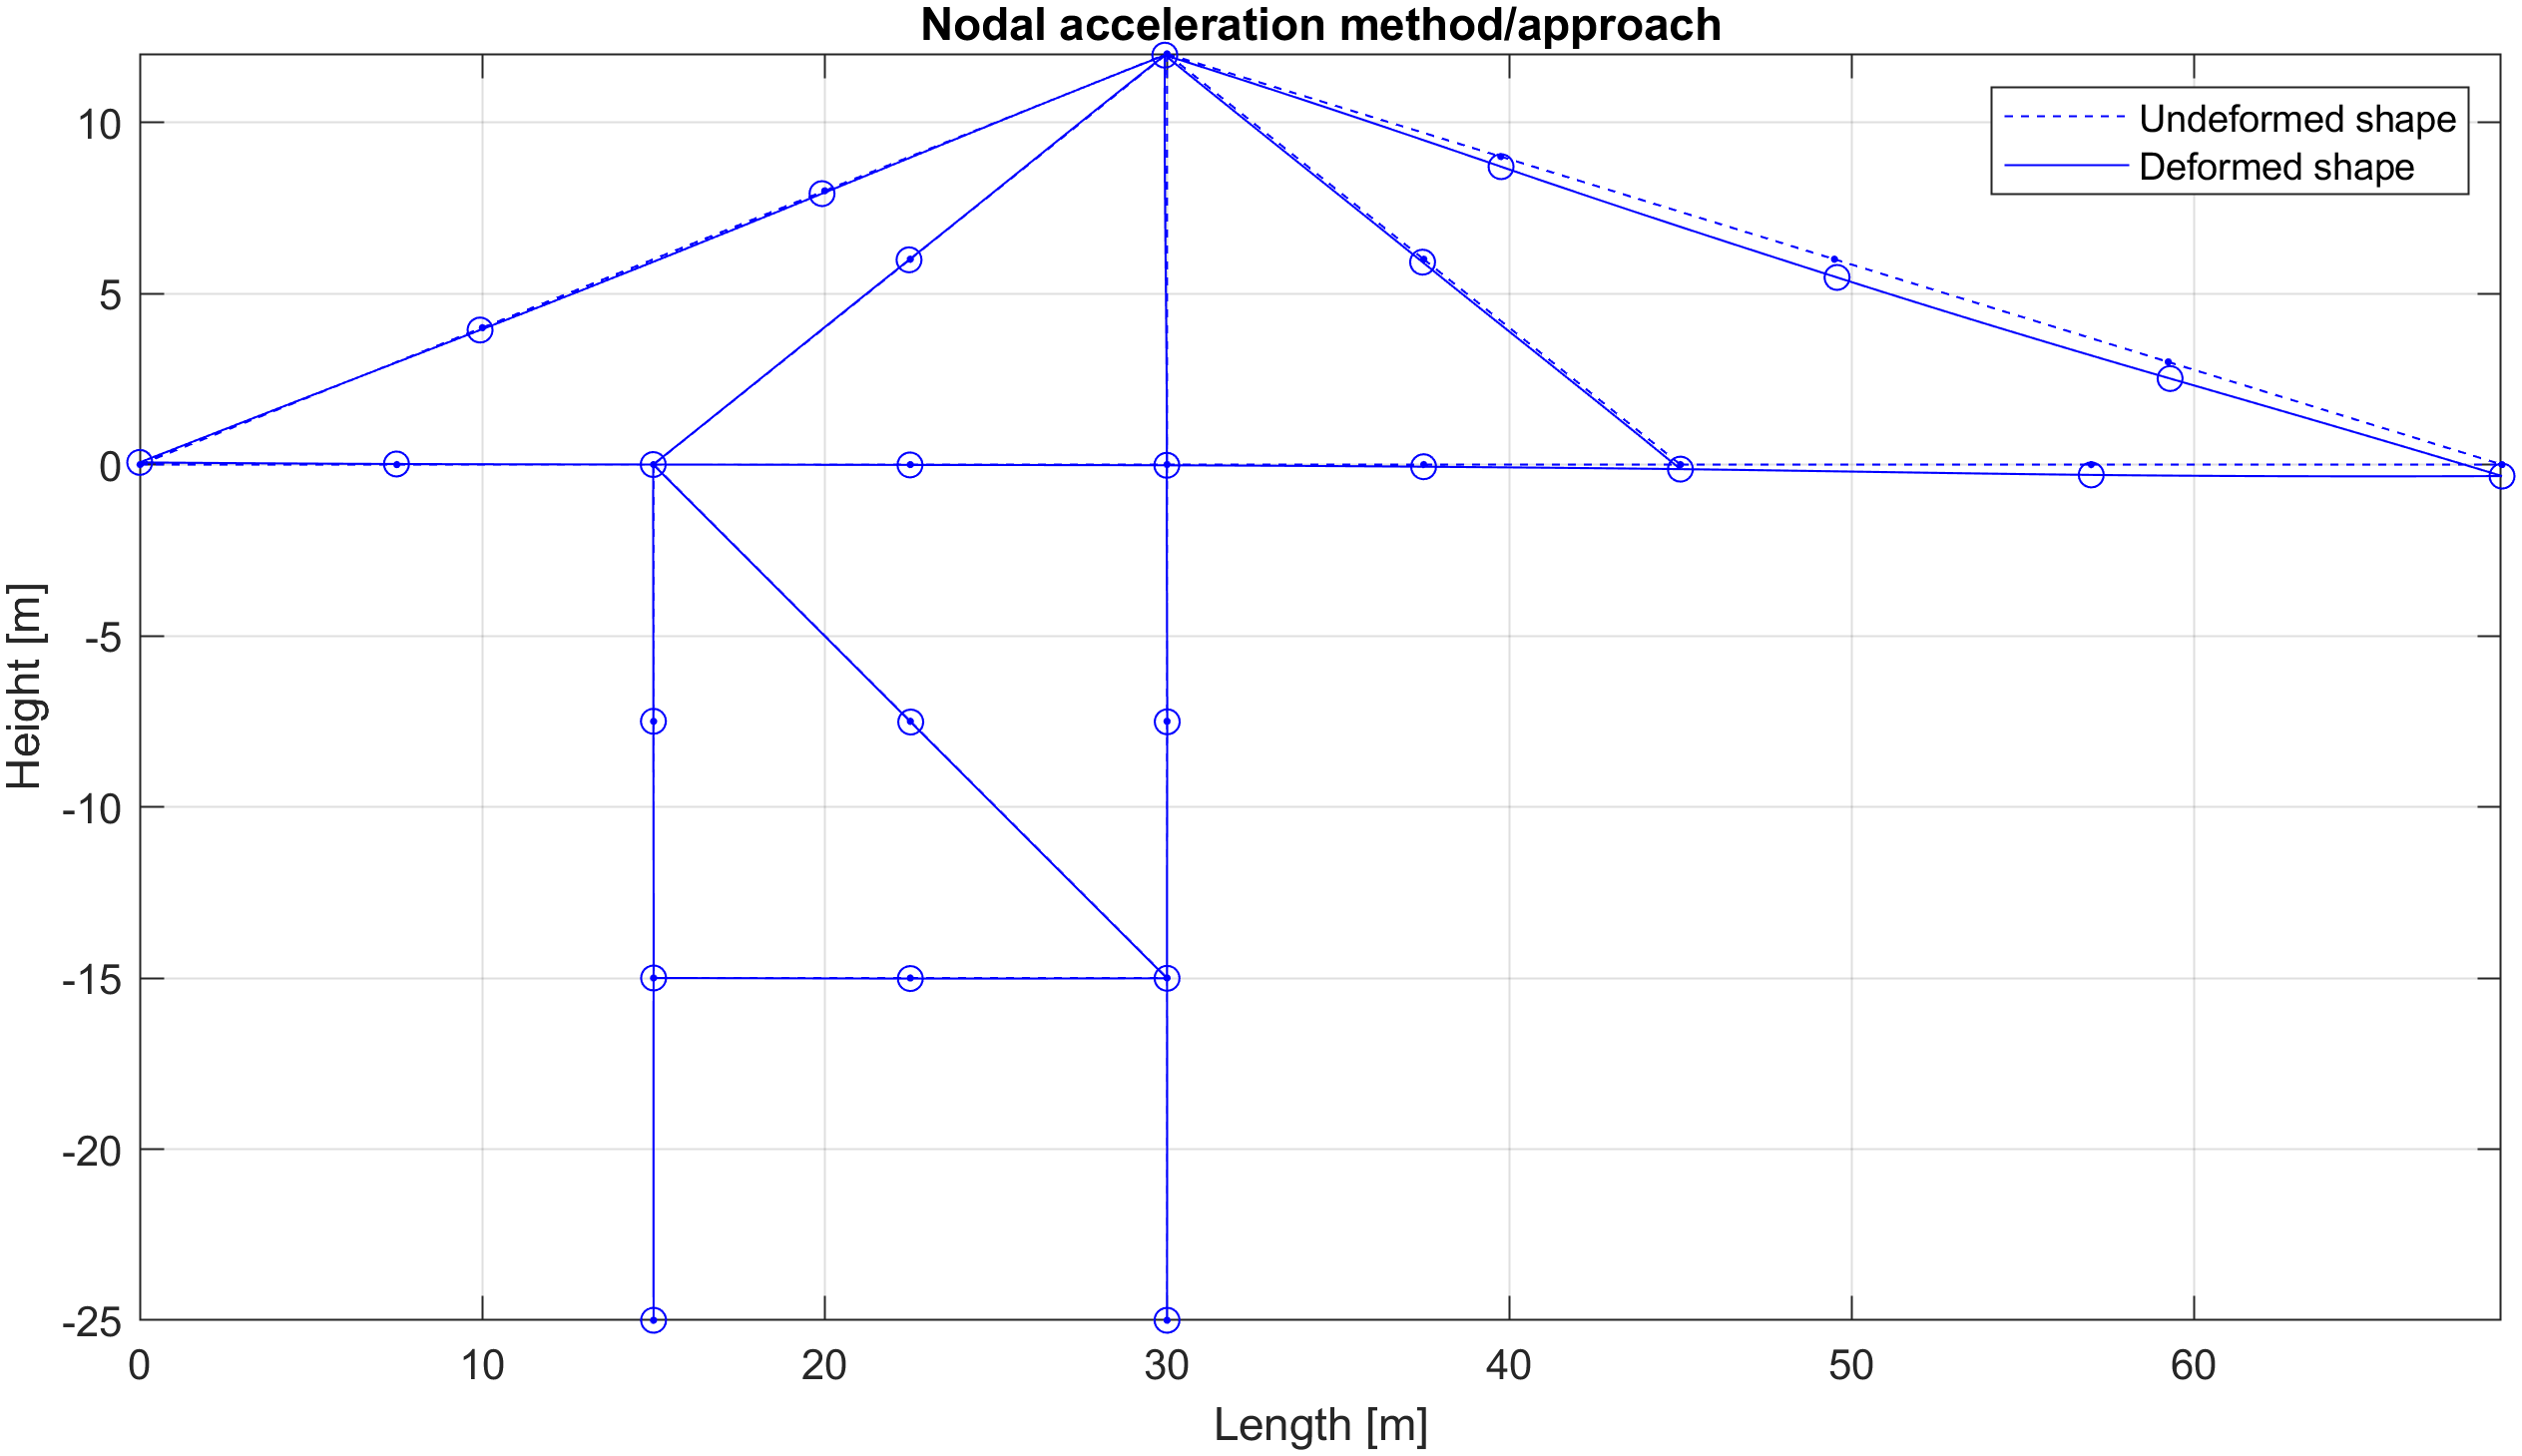
\includegraphics[width=0.45\textwidth]{img/MATLAB/Responses/Gravity_acceleration.png}
    \caption{Comparison of the static responses of the structure computed using the displacement approach and the acceleration approach.}
    \label{fig:static_responses}
\end{figure}
\section{Response due to moving loads}
\label{sec:moving_loads_response}

Finally, we can simulate a real working condition for the harbour crane, by applying a moving load on the structure.

In particular, we can consider a mass of $m = 45[T]$ moving along the $x$ axis, starting from the correspondence of node \textbf{\#7} and moving towards node \textbf{\#9} (tip of the arm crane).

\subsection{Trapezoidal motion profile}
\label{subsec:trapezoidal_motion_profile}

As for the motion type of the mass along the $x$ axis, we can consider a trapezoidal velocity profile, with a constant acceleration phase, a constant velocity phase, and a constant deceleration phase.
In particular, if we consider the total distance covered by the mass as $L = 24[m]$ and a total time of $T = 20[s]$, we can compute both the accelerations ($a_{acc} = |a_{dec}| = a$), velocity ($v_{max}$), and the time duration of each phase ($t_1$, $t_2$ and $t_3$):

\begin{equation}
    \begin{cases}
        L = \frac{1}{2} \cdot a \cdot t_1^2 + v_{max} \cdot t_2 + \frac{1}{2} \cdot |a| \cdot t_3^2 \\
        T = t_1 + t_2 + t_3
    \end{cases}
\end{equation}

By solving the system of equations, we can find the following values:

\begin{equation}
    \begin{cases}
        a = 0.25 [m/s^2]  \\
        v_{max} = 2 [m/s] \\
        t_1 = 8 [s]       \\
        t_2 = 4 [s]       \\
        t_3 = 8 [s]
    \end{cases}
\end{equation}

Once the position of the load over time is computed, we must compute the equivalent nodal forces that is applied to the structure because of the load.

For simplicity, we neglect any nodal momentum, and we just consider the vertical nodal force.
By doing so, we can compute the equivalent nodal force by solving the following equations:

\begin{align}
    \xi           & = \frac{x - x_1}{x_2 - x_1} \\
    \mathbf{F_{F, eq, left}}  & = m \cdot g \cdot \xi       \\
    \mathbf{F_{F, eq, right}} & = m \cdot g \cdot (1 - \xi)
    \label{eq:equivalent_nodal_force}
\end{align}

Where $x$ is the position of the mass, $x_1$ and $x_2$ are the position of the two nodes that are closest to the mass, and $g$ is the gravity acceleration.

Once the nodal forces are known for each time step, we can compute the nodal displacements by solving the partial differential equation that describes the motion of the structure:

\begin{equation}
    [M_{FF}] \cdot \mathbf{\ddot{X}}(t) + [C_{FF}] \cdot \mathbf{\dot{X}}(t) + [K_{FF}] \cdot \mathbf{X}(t) = \mathbf{F_{F, eq}}(t)
    \label{eq:dynamic_equation}
\end{equation}

Where $[M_{FF}]$, $[C_{FF}]$ and $[K_{FF}]$ are the mass, damping and stiffness matrices of the structure, $\mathbf{X}$ is the nodal displacement vector, and $\mathbf{F_{F, eq}}$ is the equivalent nodal force vector.

To solve the equation, we must rely on a numerical method, such as the `Runge-Kutta' method, that allows us to solve the equation for each time step.

\subsection{Initial conditions}
\label{subsec:initial_conditions}

One important aspect about this type of analysis is the initial conditions of the structure.

In particular, we can consider two different initial conditions:

\begin{itemize}
    \item \textbf{Initial condition 1}: the structure is in its undeformed configuration, and the load is suddenly added to the structure and starts moving.
    \item \textbf{Initial condition 2}: the structure is in its deformed configuration due to the static loads of the mass, which then starts to move along the $x$ axis.
\end{itemize}

As we can imagine, the first set of initial conditions will lead to a much more complex dynamic response since it will be the superposition of the fast dynamic response due to the sudden addition of the load (oscillatory behavior) and the slow dynamic response due to the moving load.
On the other hand, the second set of initial conditions will lead to a cleaner and calm dynamic response, since the structure starts from a condition much more similar to the final condition.
\subsection{Implementation}
\label{subsec:implementation}

Before proceeding with the discussion about the results, we report here the code implementation used to perform the dynamic analysis of the structure due to the moving load.

Using \texttt{MATLAB}, the code is the following:

\begin{lstlisting}[language=Matlab, caption={Implementation of the moving load dynamic analysis.}]
    load_position = @(t) ...
        (t <= t1) .*                             (1/2 * a * t.^2) + ...
        (t > t1 & t <= (t1 + t2)) .*             (1/2 * a * t1^2 + v * (t - t1)) + ...
        (t > (t1 + t2) & t <= (t1 + t2 + t3)) .* (1/2 * a * t1^2 + v * t2 + v * (t - (t2 + t1)) - 1/2 * a * (t - (t1 + t2)).^2) + ...
        (t > (t1 + t2 + t3)) .*                  (1/2 * a * t1^2 + v * t2 + v * t3 - 1/2 * a * t3.^2);

    Q_func = @(t) Phi' * compute_nodal_load(load_position(t), xy, idb, -9.81 * 40e3);

    initial_conditions = [zeros(length(Q_func(0)), 1) zeros(length(Q_func(0)), 1)];
    initial_conditions = [zeros(length(Q_func(0)), 1) K_FF_modal \ Q_func(0)];

    [t, z] = ode45( ...
        @(t, z) EquationOfMotion(t, z, M_FF_modal, C_FF_modal, K_FF_modal, Q_func), ...
        [0 max(t_vet)], ...
        initial_conditions, ...
        odeset('RelTol', 1e-6, 'AbsTol', 1e-6));

    X_moving_load = Phi * z(:, size(Phi, 2)+1:end)';

    %% Functions

    function [z_dot] = EquationOfMotion(t, z, M_FF_modal, C_FF_modal, K_FF_modal, Q_func)

        N_considered_modes = size(K_FF_modal, 1);

        q_dot = z(1:N_considered_modes, 1);
        q = z(N_considered_modes + (1:N_considered_modes), 1);

        % M * x_dot_dot + C * x_dot + K * x = F(t) -> Modal coordinates -> q
        q_dot_dot = M_FF_modal \ (Q_func(t) - C_FF_modal * q_dot - K_FF_modal * q);

        z_dot(1:N_considered_modes, 1) = q_dot_dot;
        z_dot(N_considered_modes + (1:N_considered_modes), 1) = q_dot;

    end


    function F_nodal = compute_nodal_load(load_position, xy, idb, F0)
    % Strictly related to our case at hand, nodes D to A.

        F_nodal = zeros(71, 1);

        if (load_position + xy(7, 1) < xy(8, 1))

            L = xy(8, 1) - xy(7, 1);
            xi = (load_position) / L;

            N1 = 1 - xi;
            N2 = xi;

            F_nodal(idb(7, 2)) = F0 * N1;
            F_nodal(idb(8, 2)) = F0 * N2;

        else

            L = xy(9, 1) - xy(8, 1);
            xi = (load_position - (xy(8, 1) - xy(7, 1))) / L;

            N1 = 1 - xi;
            N2 = xi;

            F_nodal(idb(8, 2)) = F0 * N1;
            F_nodal(idb(9, 2)) = F0 * N2;

        end

end

\end{lstlisting}

\subsection{Results}
\label{subsec:results}

In this section, we will show the results of the dynamic analysis of the structure due to the moving load, considering both the cases of initial conditions as explained in the previous section.

\paragraph{Initial condition 1}

In this case, the structure is in its undeformed configuration, and the load is suddenly added to the structure and starts moving at $t = 0$.

\begin{figure}[H]
    \centering
    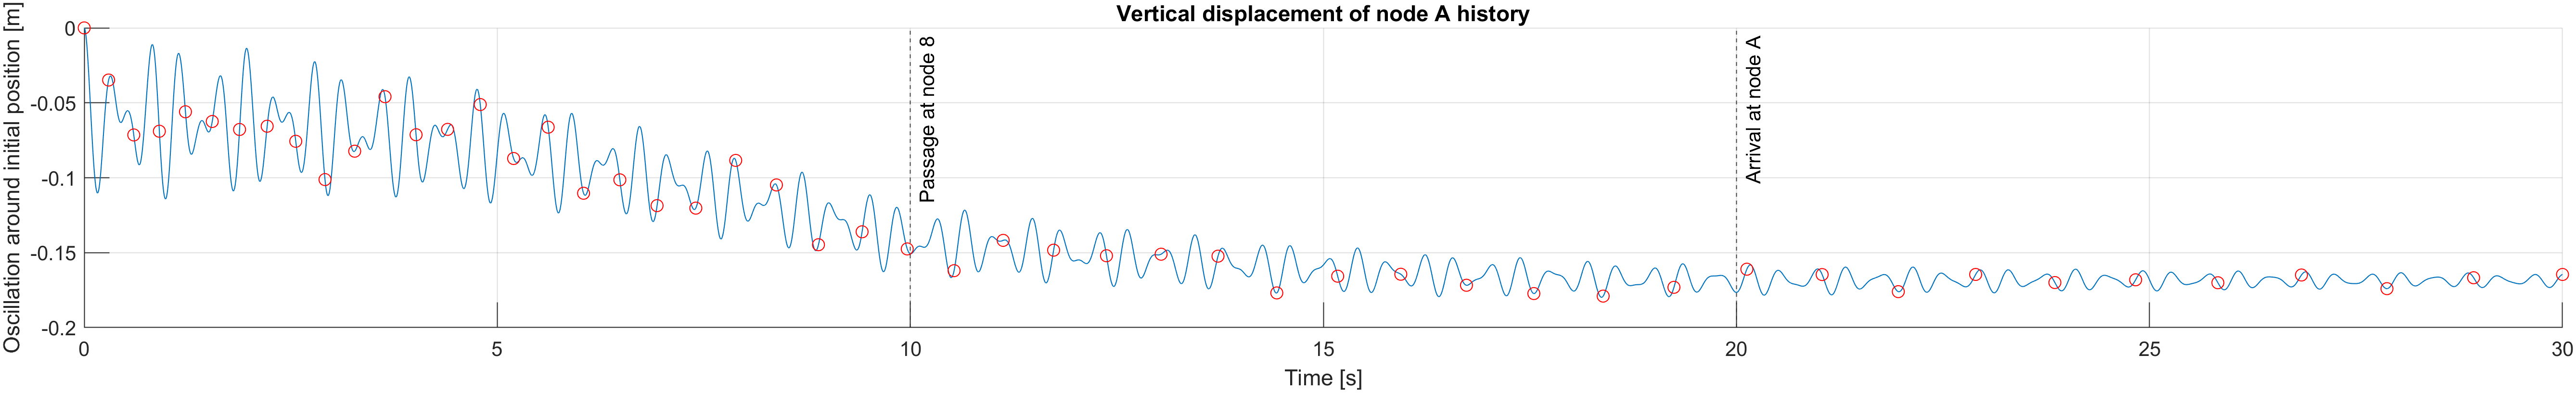
\includegraphics[width=\textwidth]{img/MATLAB/Responses/Moving_load_history_condition_1.png}
    \caption{Dynamic response of the structure due to the moving load (initial condition 1)}
    \label{fig:moving_loads_response_initial_condition_1}
\end{figure}

As we can see from the time history of node A, the structure shows a fast dynamic response due to the sudden addition of the load (in some sense this might be seen as a shock/impact response), over imposed to a slow dynamic response due to the moving load.

\paragraph{Initial condition 2}

In this case, the structure is in its deformed configuration due to the static loads of the mass, which then starts to move along the $x$ axis at $t = 0$.

\begin{figure}[H]
    \centering
    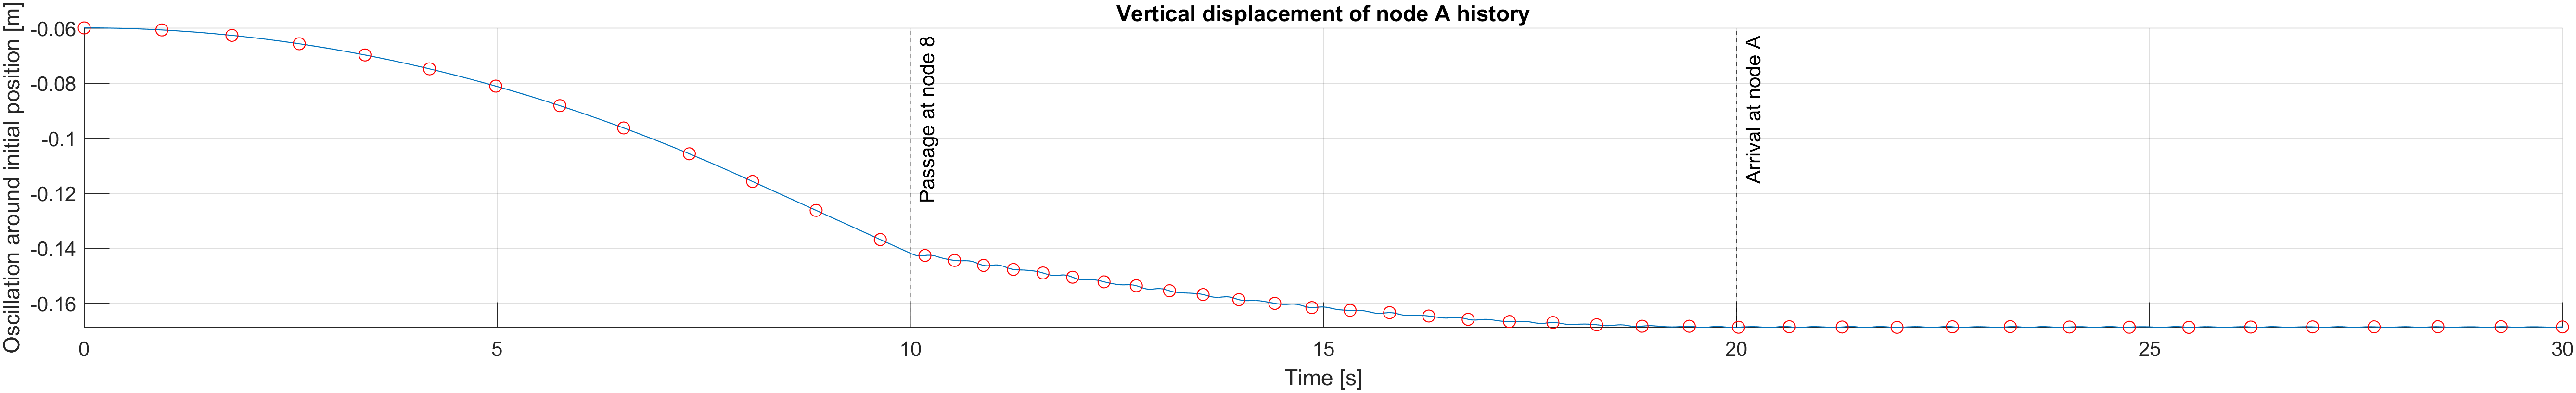
\includegraphics[width=\textwidth]{img/MATLAB/Responses/Moving_load_history_condition_2.png}
    \caption{Dynamic response of the structure due to the moving load (initial condition 2)}
    \label{fig:moving_loads_response_initial_condition_2}
\end{figure}

As we can see from the time history of node A, the structure shows a much more steady and controlled response, with no strong oscillatory behavior.
This can be explained by the absence of the equivalent shock/impact response due to the sudden addition of the load.


% \section{Conclusions}
\label{sec:conclusions}

The present work aimed at investigating the drag coefficient of a model rocket using computational fluid dynamics.

The rocket was at first modeled in an external CAD software and then imported into Ansys Fluent for the CFD simulation.
The simulation was carried out using the $k-\omega$ SST turbulence model and in a steady-state regime and the drag coefficient ($C_d$) was calculated at $85\%$ of the speed maximum speed reached by the rocket during the real world flight.

The results obtained from the CFD simulation were compared to the flight data and the simulation from \texttt{OpenRocket}, showing a good agreement with both of them after some adjustments to the thrust curve.

Moreover, the drag coefficient was found to be $C_d = 0.86$, which is in line with the expected values for a model rocket.
This value is also in line with the one obtained from the flight data and the one from \texttt{OpenRocket}.

The present work showed that CFD simulations can be a powerful tool to investigate the aerodynamic behavior of model rockets and that the results obtained can be potentially used to optimize the design iterating backward and forward between the CAD model and the CFD simulation.

% \clearpage
% \bibliographystyle{plain}
% \bibliography{ref}

\end{document}
